\documentclass[a4paper,11pt]{report}

\bibliography{main}
\bibliographystyle{unsrt}

\usepackage{fullpage}
\usepackage{graphicx}
\usepackage{wrapfig}
\usepackage{setspace}
\usepackage{float}
\usepackage{sectsty}
\usepackage{url}
\usepackage{amssymb}
\usepackage{bbm}
%\usepackage{latexsymb}%

\graphicspath{{./figures/}}

\chapterfont{\LARGE}
\sectionfont{\large}

\setcounter{secnumdepth}{0}

\floatstyle{boxed}

\newfloat{formality}{H}{lop}

\doublespacing
\author{Daniel Demby}
\title{Final Year Dissertation}
\begin{document}
\begin{titlepage}
 
\begin{center}
 
 
% Upper part of the page
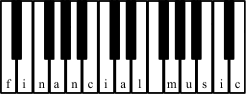
\includegraphics[scale=0.5]{./logo}\\[1cm]

\textsc{\Large School of Mathematical and Computer Sciences}
\textsc{\LARGE Heriot-Watt University}\\[1.5cm]
 
\textsc{\Large Final Year Dissertation}\\[0.5cm]

%\textsc{\Large Final Version}\\[0.5cm]
 
 
% Title
{ \huge \bfseries Financial Music}\\[0.4cm]

\vfill

% Author and supervisor
\begin{minipage}{0.4\textwidth}
\begin{flushleft} \large
\emph{Author:}\\
\textsc{DANIEL DEMBY}
\end{flushleft}
\end{minipage}
\begin{minipage}{0.4\textwidth}
\begin{flushright} \large
\emph{Supervisor:} \\
Prof. \textsc{DAVID CORNE}
\end{flushright}
\end{minipage}
 
\vfill
 
\vfill

\vfill
 
% Bottom of the page
{\large \today}

\end{center}
 
\end{titlepage}
\thispagestyle{empty}
\begin{quote}
Declaration: \\

I, Daniel Demby, confirm that this work submitted for assessment is my own and is expressed in my own words. Any uses made within it of the works of other authors in any form eg: ideas, figures, text, tables, programs are properly acknowledged at any point of their use. A list of the references employed is included. \\

Signed: \_\_\_\_\_\_\_\_\_\_\_\_\_\_\_\_\_\_\_\_\_\_\_\_\_\_\_\_\_\_\_\_\_ \\

Date: \_\_\_\_\_\_\_\_\_\_\_\_\_\_\_\_\_\_\_\_\_\_\_\_\_\_\_\_\_\_\_\_\_\_\_ \\
\end{quote}
\begin{abstract}
\thispagestyle{empty}

\noindent In Douglas Adams' novel `Dirk Gently's Holistic Detective Agency', he describes software capable of generating music from corporate accounts. The music generated was capable of conveying the state of an account, to the point where a listener was able to make an investment decision. \\

\noindent Over the course of this dissertation, we will design, develop, implement and evaluate two approaches towards achieving this. We will focus on both conveying the account's nature, and on making the audio output as musical as possible. The first approach explored uses an mathematical approach in which we generate `signals' from the accounts. These signals to appropriate musical sequences. The second approach uses L-Systems to generate music from these same signals. \\

\noindent We will discover in the evaluation that both approaches produce audio output which is considered musical. We will also discover that the L-System approach show's the highest level of success when conveying the nature of an account. \\

\noindent Finally, we will go forward to design a novel idea called \textit{The Financial Genome}, in which we attempt to use a biologically inspired approach to identify patterns in accounts, find an optimum genome.

\end{abstract}
\begin{singlespace}
\renewcommand{\abstractname}{Acknowledgments}
\begin{abstract}

\noindent David Corne, who presented such a compelling dissertation topic, and agreed to take me on. \\

\noindent Gerard Briscoe, for proof-reading the chapters and explaining many of the intricacies of LaTeX to me. \\

\noindent David Demby, for analysing the accounts for me and providing an insight into accountancy and finance that I lacked. \\

\noindent Mike Chantler, for providing useful and constructive feedback. \\

\noindent Finally, the late Douglas Adams, who came up with the original idea of generating music from accounts. \\\\

\noindent This document was composed in \LaTeX\, and processed using MiKTeX 2.7.

\end{abstract}
\thispagestyle{empty}
\tableofcontents
\thispagestyle{empty}
\end{singlespace}

\begin{singlespace}
\listoffigures
\end{singlespace}

\pagenumbering{roman}

\chapter{Introduction}
\pagenumbering{arabic}
\begin{quote}
``By the time you've sorted out a complicated idea into little steps that even a stupid machine can deal with, you've certainly learned something about it yourself.''\begin{flushright}-- Douglas Adams\end{flushright}
\end{quote}

\noindent In Douglas Adams' book \textbf{Dirk Gently's Holistic Detection Agency}, a talented software developer named Richard Macduff develops a spreadsheet programme named \textit{Anthem} with a unique feature; It can turn account data into music.

The book was written in a year when the \textit{Apple Macintosh Plus} was considered state-of-the-art technology, and Douglas Adams was clearly captivated by the potential of what kinds of programs could be created. Would the computer limit the bounds of a programmer's imagination, or allow its programmer to realise ideas that appear seemingly impossible?

Nowadays, Digital on-the-fly music generation is becoming increasingly popular for many different applications, so perhaps Adams' idea doesn't seem so far-fetched anymore. In the entertainment industry, games such as Electroplankton allow the dynamic generation of music based on the actions of fictional organisms.\footnote{\url{http://electroplankton.nintendods.com}} Conversely, some games work the other way round, generating levels from music. Audiosurf is one such example, generating racing tracks from the user's MP3 collection.\footnote{\url{http://www.audio-surf.com}}

However, to my knowledge, no one has attempted to implement Adams' idea\ldots until now.

\section{Motivation and Objectives}

In theoretical computer science (computability theory), we talk about a problem having a certain level of complexity. In other words, some problems can be solved by a computer, some can't, and for some we just don't know. Whilst this concept doesn't directly apply to this dissertation topic (we're not looking at directly solving a mathematical problem per se), it may make us wonder about solving a problem with a computer where the end result is dependant on human opinion.\footnote{Donald E. Knuth published a surreal paper entitled ``The Compexity of Songs'' in 1984, implying that songs had complexity levels similar to those of problems in the computability theory. \url{http://www.cs.utexas.edu/arvindn/misc/knuth_song_complexity.pdf}}

This is one of the fundamental challenges posed by this project; Can we solve a problem (generating music from accounts) whereby our success measure (that the music represents the account's nature) is dependant on human subjectivity?

The analysis of a company's account by an expert (such as an accountant) is a logical process, and one that may take some considerable skill. Therefore, an account given to any number of experts to analyse will almost always conclude with a unanimous opinion as to the account's condition.

Music is different. When a piece of music is played to a group of people, there often will \textit{not} be a consensus of opinion as to the meaning of a piece of music. This in its self provides the challenge of taking something of an objective perception (raw account data), and presenting its meaning using something of a subjective perception (music).

An equally fundamental challenge that we will encounter is how to take two disparate concepts with seemingly little in common (accounts and music), and then link them together with tangible ideas which can be implemented and evaluated.

From these challenges, the ultimate aim of this project (this project's `holy grail') is to produce note sequences from accounts which both \textbf{convey the state of the account} and also \textbf{sound like well structured pieces of music}. Along the way, we will hope to learn some interesting and surprising things from the issues we encounter.

\section{Dissertation Outline}

The structure of this dissertation follows a natural flow from one idea to another. Where appropriate, we discuss the origin, design and implementation of a single idea in the same chapter.

In \textbf{Chapter 2}, we will begin by looking at the theory underpinning the project. What is a financial statement? What are the fundamentals of music cognition, and why are they so important in this dissertation?

With \textbf{Chapter 3}, we will look the design and implementation of a central software architecture capable of reading accounts, and playing music. We will also look at how implementations of ideas discussed in this project will connect to this crucial framework.

In \textbf{Chapter 4} and \textbf{Chapter 5}, we will consider in detail two approaches to generating music from accounts. The first, \textbf{Signal Mapping}, takes a mathematical approach. The second, \textbf{L-System Music Generation}, comes from a Biologically-Inspired direction. Both of these approaches will be followed through from conception, to design and finally to an implementation, using the architecture discussed in the second chapter.

In \textbf{Chapter 6}, we will evaluate these two approaches to determine how successful they have been. The evaluation will use human testers, and the evaluation technique will especially consider the subjective nature of music interpretation. The results of the evaluation will be carefully analysed, and some interesting conclusions will be drawn.

In \textbf{Chapter 7}, we will propose a more ambitious approach called \textbf{The Financial Genome}. This idea presents a method by which unique features of an account can be indentified through a combination of supervised machine learning and evolutionary algorithms. We will see how the approach used for evaluating the first two implementations naturally leads to this approach.

Finally, in \textbf{Chapter 8}, we will conclude and look at avenues in which the project could potentially be expanded on beyond its current scope in the future. We will look at questions raised during the implementation process, and evaluate the project as a whole.

\chapter{The Theory}

In this chapter, we will look at some of the theory underpinning this project. We will discover how company accounts are formed, and we will look at how music cognition relates to how people perceive music.

\section{Company Accounts Analysis}

IA company's account consists of three main statements. They are the \textbf{Balance Sheet}, the \textbf{Income Statement} and the \textbf{Cash Flow Statement}.\footnote{\url{http://www.flexinvest.co.uk/secrets.htm}}

The \textbf{balance sheet} gives an impression of a company's situation at a specific point in time. If we compare two balance sheets that are a year apart, we can determine useful details about the company's performance over the year, and the current direction that it is heading. Here is an example of what a company's balance sheet looks like (amounts are given in millions of US Dollars):

\small
\begin{center}
\begin{singlespace}
\begin{tabular}{ | l || l | l | l | l | l | }
\hline
 & \textbf{Current Assets} & \textbf{Total Assets} & \textbf{Current Liabilities} & \textbf{Total Liabilities} & \textbf{Total Equity} \\ \hline \hline
2006 & 4076.71 & 9251.8 & 3150.2 & 8401.05 & 850.13 \\ \hline
2007 & 3766.27 & 8342.6 & 5912.8 & 7821.86 & 520.74 \\
\hline
\end{tabular}
\end{singlespace}
\end{center}
\normalsize

Of the remaining two statements, The \textbf{profit and loss statement} records how the company's profit and losses were reached over the course of a year, and the \textbf{cash flow statement} shows movements in cash and cash equivalents (assets). As we are going to be using snapshots of a company's state at points in time, we will keep our focus on the balance sheet as the source for deriving music.

\section{Music Theory}

Music Theory is the field of study which explains the mechanics of music, and there are some specific ideas that we will need to be very familiar with in order to develop ideas for Financial Music.

\begin{singlespace}
\begin{formality}
\subsection*{Melody}

A melody is a successive sequence of notes. If the sequence is well structured within a scale, it will sound musical and pleasant to the ear.

\subsection*{Key}

A key has a signature (major or minor) and a tonic (the root note).

\subsection*{Octave}

An octave is a distance of twelve successive notes between two successive musical pitches.

\subsection*{Scales}

A scale is a sequence of notes within a key. For example, a major scale is given as the following notes in an octave: $[1, 3, 5, 6, 8, 10, 12]$.

\subsection*{Chords}

Several notes played concurrently within the same key. Chords add depth to music when complementing a melody.

\subsection*{Clashing Notes}

Two or more notes played concurrently, of which at least two are in different keys. The sound is discordant.
\end{formality}
\end{singlespace}

\section{Music Cognition}

Music cognition is a field of study which concerns its self with how the human mind perceives music. This is a crucial area to understand before beginning the design process, as we need to know what kind of music to generate to create a certain impression in the listener.

Music cognition consists of several sub-topics, and in this project, we are particularly concerned with the topic of music perception.

Music perception is the process by which the \textbf{past experience} of a listener processes \textbf{sounds} in to \textbf{music}.\footnote{Note that as the experience of the listener will determine the impression given by a piece of music, it may be that a listener's cultural musical background may effect how well we can convey an account's nature to them through the music. This concern is beyond the scope of this project, and is further discussed in the \textit{Further Work} section in the final chapter.} Musical elements that the listener's brain is capable of perceiving include pitch, rhythm and tonality.

Tonality is an important musical element to consider, as it can convey \textbf{emotion}, triggering different areas of the brain depending on the emotion being conveyed. This is a feature that we can apply in designing Financial Music, as we can use tonality to convey the nature of an account in this way.

\section{The MIDI Standard}

MIDI is an acronym for \textbf{Musical Instrument Digital Interface}. Developed in 1983, it is a versatile protocol for communicating musical sequences and instrumentation. MIDI data consists of a number of \textbf{channels}, which contain lists of integer values to represent notes. Channel contents can be played (or transmitted) concurrently, resulting in music.

The most commonly used implementation of MIDI is known as \textbf{Genral MIDI}, and it is this version that we will be utilising. MIDI is a good choice for representing music in this project, as we can easily write algorithms to generate the sequences of integers needed to play music using this standard. MIDI is also very well supported, and class libraries are available for many programming languages which allow the playing of MIDI sequences with ease.

\section{First Case Study: Playing the Market}

An experimental music project named \textit{Emerald Suspension}\footnote{The homepage of Emerald Suspension can be found at: \url{http://www.emeraldsuspension.com}} produced an album titled ``Playing the Market'', which uses patterns derived from stock market movements to inspire interesting music, which was then further arranged by the musicians. A soundbite from their website declares the following:

\begin{quote}
``Conceptual audio arrangements by Emerald Suspension are structured based on patterns created by the stock market, economic indicators, algorithms, and other data sources.''
\end{quote}

\noindent The \textit{Playing the Market} project differs somewhat from Financial Music in that \textit{Emerald Suspension} are using movements in the \textit{stock market} as a template to produce music for artistic reasons. The data they used to generate the music was specifically chosen because it resulted in good music. The music produced was then refined by the musicians to a high standard.

In Financial Music, we will be using \textit{company accounts} to generate music for \textit{any} account. As there will be no artistic selection of musical output, we will need to develop a way of generating music for any given account in real time. There will also be no refining of the output; the music produced must stand on its own merits.

We can draw inspiration from Emerald Suspension's project. Their album demonstrates that there \textit{are} distinct patterns in the financial world, which can be used to generate music. They also demonstrate that the music generated from these patterns can be perceived by listeners to have a meaning which represents the original patterns.

\section{Summary}

So far, we have seen how a company's accounts are represented. We have looked at issues of music cognition, and seen how these issues will play a part in our approach towards a design.

With a basic understanding of the issues of the financial statement and music cognition, we are now in a position to think about drawing connections between these two eclectic concepts. But, before we do this, we need to design and implement an appropriate software architecture, and it is this that we will look at in the next chapter.

\chapter{Software Architecture}

In this chapter, we will consider the \textbf{general requirements} of a program which will turn accounts into music. At this stage we do not know the specifics of how this will be achieved, therefore the architecture needs to be as versatile as possible.

We will see how we can split the software into two distinct sections. One will handles the input and output operations. the other will do the actual processing to produce music from accounts.

Additionally, the architecture will support a ``plug-in'' framework, allowing many different implementations to be attached with ease.

\begin{figure}[ht]
\centering
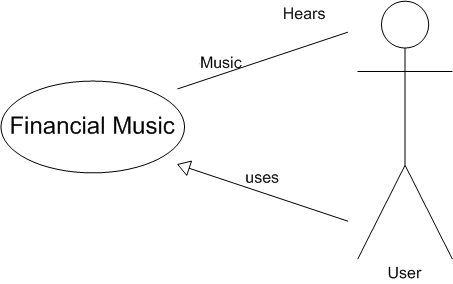
\includegraphics[scale=1.2]{use_case}
\caption{Use case diagram, demonstrating the relationship between the user and the software.}
\label{fig:use_case}
\end{figure}

\section{Requirements of the Framework}

The framework must meet the following requirements:
\begin{enumerate}
\begin{singlespace}
\item Input:
\begin{enumerate}
\item Ability to import accounts from a standard format.
\item Simplicity to add additional methods of importing accounts.
\end{enumerate}
\item Output:
\begin{enumerate}
\item Output in a common music format.
\item Ability to play music.
\end{enumerate}
\item Easy addition of core modules for different methods of generating music from accounts.
\item Versatile framework to allow for high levels of experimentation during development.
\end{singlespace}
\end{enumerate}

\section{The Shell and the Core}

Recall that we mentioned that parts of the software can will fall into two distinct categories. We will term these categories the \textbf{Shell} and the \textbf{Core}. The Shell deals with \textbf{input and output} (I/O) operations such as reading in accounts (input), dealing with file operations (input and output) and playing the music (output).

The Core is where the process of turning accounts into music takes place, and therefore performs the \textbf{processing}.

Looking at the software in this way is essential, as we do not wish to be concerned with issues of input and output (worrying about where the data is coming from or going to) while we are designing processing strategies. Therefore, we should set things up so that the Core doesn't need to be concerned with where the account data is coming from, or what to do with the music that is produced \textit{(figure \ref{fig:shellcore})}.

\begin{figure}[ht]
\centering
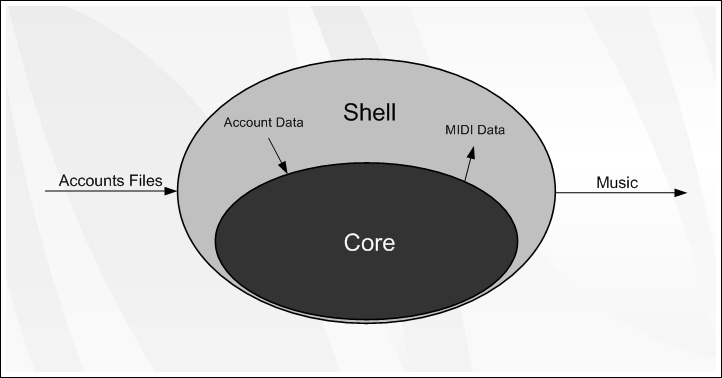
\includegraphics[scale=1.5]{shellcore}
\caption{The relationship between the Shell and the Core in the software's architecture.}
\label{fig:shellcore}
\end{figure}

\section{Languages of Implementation}

Given the differing natures of the Shell and the Core, it is necessary to carefully select a language of implementation that will best suit each task. 

The language chosen for implementation of the Shell is \textbf{Java}. Java is a popular high-level programming language. It also has the advantage of being cross-platform, and web capable.

Java is a suitable language for the tasks the Shell will have to perform, as it has a good selection of class libraries at its disposal for dealing with all the I/O operations that will be required by this project. It has libraries for reading and parsing files. It also has excellent MIDI capabilities.

The Core is concerned purely with mathematical and logical operations which will turn accounts into music, and therefore requires a language which has a syntax oriented towards this end. A functional programming language is a good choice for this, and \textbf{Python} was chosen for this purpose. Python is a high level dynamically typed language, with support for lists, sets and tuples. It supports a functional programming paradigm, inspired by languages such as SML and Haskell. As we will be presenting designs which will be expressed formally, this paradigm will allow focus on the actual processes involved in music generation.

Taking a functional programming approach to writing the core moudules is useful, as it allows us to abstract a problem down to a state where each element of a problem has its own function. This in turn allows the sharing of functions across problems which share many of the same elements.

It also allows functions to be tested individually as they are written. This way, debugging the program is a simpler process; If the integrity of the modules can be verified, then the interactions between modules can be studied in isolation.

(It should be noted however, that the functions developed on the coming pages often display \textit{side-effects} such as displaying text on screen or accessing a global variable, therefore some may not consider the approach truly functional)

As a final point, we need the language used for the core to be able to communicate transparently with the shell. To this end, the core is really implemented in \textbf{Jython}, which is an implementation of the Python language using the \textbf{Java Virtual Machine}.\footnote{The Jython website can be found at: \url{http://www.jython.org}}

\section{Modules of the Shell}

Recall that modules in the shell are responsible mainly for I/O operations, and will be implemented in Java. There are three main classes involved in this:

\begin{itemize}
\begin{singlespace}
\item \texttt{AccountReader.class} -- Reads in the accounts from source files.
\item \texttt{PlayMusic.class} -- Plays music when given a 2 dimensional integer array of MIDI values.
\item \texttt{MusicReader.class} -- Looks for a CSV file with MIDI values and pipes it to \texttt{PlayMusic.class}.
\end{singlespace}
\end{itemize}

\section{Modules of the Core}

Core modules deal with the actual processing. They are as follows:

\begin{itemize}
\begin{singlespace}
\item \texttt{Shared.py} -- Contains functions shared across modules in the Core.
\item \texttt{Settings.py} -- Contains global settings in one location, for easy access.
\item \texttt{Mapping.py} -- Contains function for the Signal Mapping implementation (Chapter 4).
\item \texttt{LSS.py} -- Contains function for the L-System Music Generation implementation (Chapter 5).
\item \texttt{Linden.py} -- Contains functions to implement a generic L-System (also Chapter 5).
\item \texttt{Genome.py} -- Contains functions for the Financial Genome approach (Chapter 7).
\end{singlespace}
\end{itemize}

\section{Module Interactions and Data Flow}

The interactions between modules can be observed in \textit{figure \ref{fig:UML}}.

\begin{figure}[ht]
\centering
\includegraphics[scale=1.5]{UML}
\caption{A UML representation of the interaction between modules in Financial Music.}
\label{fig:UML}
\end{figure}

\section{Platform Requirements}

A system running \textit{Financial Music} will need to meet the following minimum requirements:

\begin{enumerate}
\begin{singlespace}
\item Hardware
\begin{enumerate}
\item MIDI Capabilities
\end{enumerate}
\item Software
\begin{enumerate}
\item Java 1.6.0
\item Jython 2.2.1
\end{enumerate}
\end{singlespace}
\end{enumerate}

\section{Summary}

In this chapter, we have designed and constructed a software architecture to support Financial Music. With a Shell (implemented in Java) and a Core (Implemented in Jython), it will be capable of reading in accounts from an external source, and of playing music using the MIDI standard.

As we develop Python code in the future chapters, we will see an evolution of the Core. However, the Java code of the Shell will remain unchanged, and unaffected by development in the Core.

With a framework in place, we are now ready to begin developing approaches to turning accounts into music, and the next couple of chapters will explore two approaches towards achieving this.

\chapter{Approach 1: Signal Mapping}

The first approach we will develop is an idea called \textbf{Signal Mapping}. Accounts have attributes, and when we look at the accounts for two subsequent years, we can observe changes in these attributes. We will see that from these changes, we can derive signals, which can be mapped to appropriate musical constructs. These constructs can be arranged together to form music. To do this, we will be working with the account \textbf{balance sheet}.


\section{Notation and Definitions}

\begin{center}
\begin{singlespace}
\begin{tabular}{ l l }
\hline
\hline
\textbf{\{ $\ldots$ \}} & A set of items \\ \hline
\textbf{Sequence} & An ordered set which can contain repeating elements \\ \hline
\textbf{List} & Another name for a Sequence \\ \hline
\textbf{$\langle \ldots \rangle$} & A sequence of items \\ \hline
\textbf{Musical sequence}: & A finite sequence of notes. \\ \hline
\textbf{Set of musical sequences}: & Multiple musical sequences whose feel is governed by the set of \\
 & musical attributes. \\ \hline
\textbf{Musical attribute}: & A static value which pre-determines the feel of a musical sequence. \\
 & For example: tempo, time signature or key signature. \\ \hline
\textbf{Set of musical attributes}: & Multiple non-contradicting musical attributes. \\ \hline
\textbf{Musical movement}: & The set of musical sequences as governed by the set of musical \\
& attributes \textit{(i.e. the complete music generated by the accounts)}. \\ \hline
\hline
\end{tabular}
\end{singlespace}
\end{center}



\section{Problem Discussion}

Recall that an account's balance sheet consists of five attributes. Recall also that to assess the health of a company, we can compare the balance sheets between two subsequent years.

Now consider the diagram given in \textit{figure \ref{fig:ss01}}. We can connect two parameters together to produce a unique \textbf{signal}. This signal can then be routed to a \textbf{processor}, which converts it into a musical sequence. Continuing onwards by piping the output signals of multiple processors produces a complete movement of music. By tweaking and fine tuning the settings of these processors, we can harness the sound so that it represents the account's data.



\begin{figure}[ht]
\centering
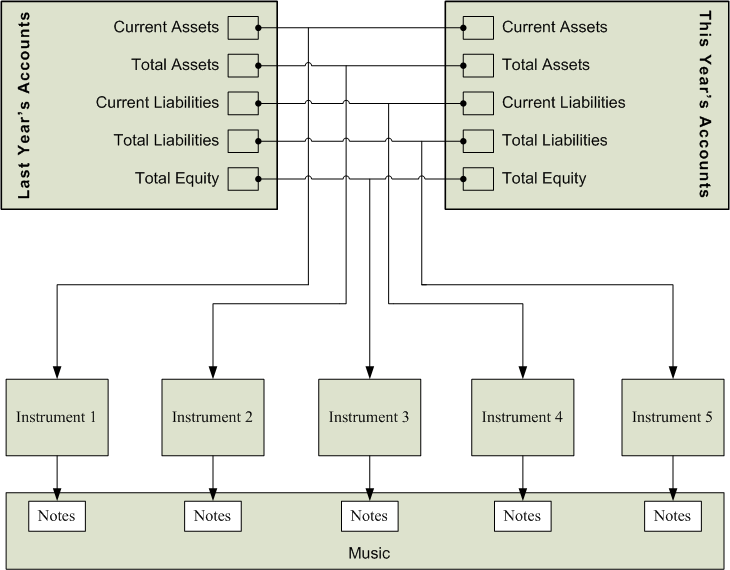
\includegraphics[scale=0.5]{ss01}
\caption{Mapping of account information to music. Each item of the account is independently mapped to a musical sequence.}
\label{fig:ss01}
\end{figure}

\noindent Essentially, we are mapping the difference between two parameters to a musical sequence or musical attribute. The processors are `black boxes', and the overall picture is only concerned with the signals going in and out of the processors. In other words, each processor will correspond to a function in the program.

Looking inside one of these processors, there would be an algorithm to take the account values and turn them into a suitable musical sequence. The processors will have `dials' which when modified change variables within the algorithm. It is these settings that we will tweak to fine tune the system, so that it produces the musical output we are looking for.



\section{Processor Isolation: A Sequential Approach}

The most crucial issue we are concerned with is that the overall sound produced must reflect the overall state of the accounts.  Although we are mapping individual account details to individual musical elements, we have to ensure that the overall �feel� of the sound fits the overall state of the accounts. 

The first approach we will try is to have each signal routed to an isolated processor. This processor generates a musical sequence. These sequences are played sequentially, one after the other. The result is a musical sequence in the form of a melody, which gives an impression of the account.

As some changes are more significant than other changes (bigger change in values of account attribute between years), we order the signals in terms of \textbf{magnitude}. This way, the individual musical sequences are joined up in order of importance.

We also need a way of deriving musical attributes which affect the \textit{whole} musical sequence. To do this, we calculate a \textbf{compound signal} which represents the overall signal spread.


\begin{figure}[ht]
\centering
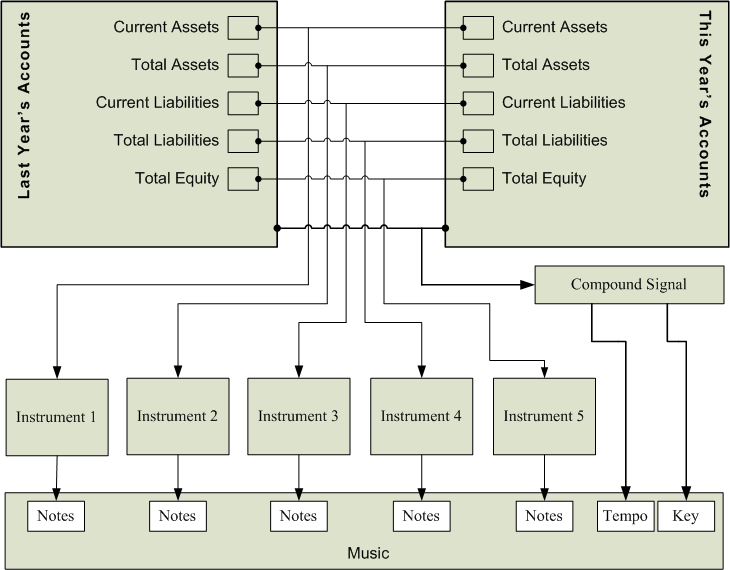
\includegraphics[scale=0.5]{ss02}
\caption{Mapping with a compound signal to control tempo and key. The compound signal is derived from the set of individual signals.}
\label{fig:ss02}
\end{figure}

\noindent 



\section{Processor Interaction: A Parallel Approach}

With the ability to play several musical sequences in sequence, we can modify this approach to produce music where the sequences play concurrently \textit{(figure \ref{fig:ss03})}. Taking this approach has the advantage of creating a completely different sound to the sequential approach, which we can compare with later.

\begin{figure}[ht]
\centering
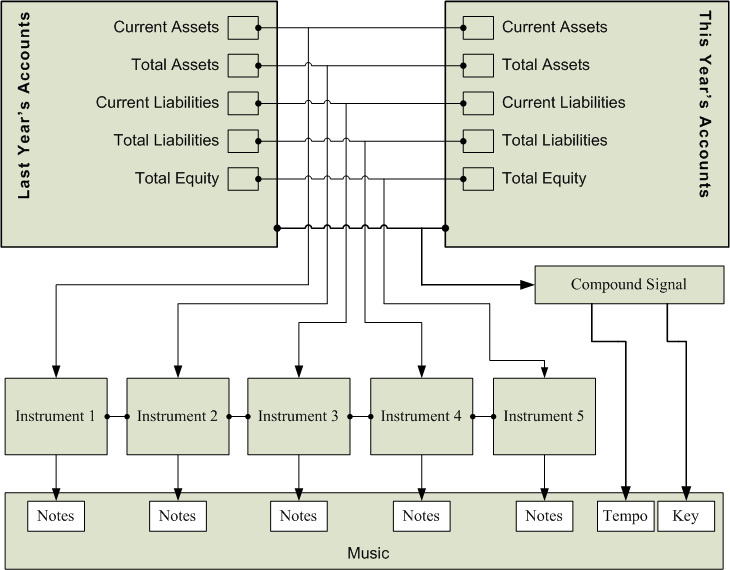
\includegraphics[scale=0.5]{ss03}
\caption{Mapping with sequences in parallel.}
\label{fig:ss03}
\end{figure}

\noindent However doing this presents us with a new problem. As each of the note sequences generated by the processors are in their own key, if we attempt to play them together, there will note clashes and general discordance of notes. Seeing as we are aiming to generate \textit{music}, this situation is clearly undesirable, and so we need a strategy to account for this. As an example, let's take the following two arbitrary note sequences:

\begin{singlespace}
\begin{formality}
$Seq_{1} = \langle C\#, F, A\# \rangle $ \\
$Seq_{2} = \langle E\#, F\#, C \rangle $
\end{formality}
\end{singlespace}

Some of these notes will clash if the sequences are played in parallel (for example, the 2nd item in each list). Additionally, if we are to adhere to a proper musical structure, we need an overall key to which all sequences should reside in.

To solve this problem, we invent the concept of a \textbf{keymap}. A keymap is a list of allowed notes, and will usually specify a scale of notes in the overall key. For example, consider the scale of C major:

\begin{singlespace}
\begin{formality}
$KeyMap = \langle C, D, E, F, G, A, B \rangle$
\end{formality}
\end{singlespace}

\noindent We map the notes of $Seq_{1}$ and $Seq_{2}$ to the notes in $KeyMap$ via the following algorithm:

\begin{singlespace}
\begin{formality}
\begin{itemize}
\item[\textbullet] \texttt{For each Note in Seq:}
	\begin{itemize}
	\item[\textbullet] \texttt{If Note not in KeyMap then:}
		\begin{itemize}
		\item[\textbullet] \texttt{If Note - 1 in KeyMap then:}
			\begin{itemize}
			\item[\textbullet] \texttt{Note = Note - 1}
			\end{itemize}
		\end{itemize}
		\item[\textbullet] \texttt{else:}
			\begin{itemize}
			\item[\textbullet] \texttt{Repeat until Note in KeyMap:}
				\begin{itemize}
				\item[\textbullet] \texttt{Note = Note + 1}
				\end{itemize}
			\end{itemize}
	\end{itemize}
\end{itemize}
\end{formality}
\end{singlespace}

\noindent Running the algorithm would re-map $Seq_{1}$ and $Seq_{2}$ as follows:

\begin{singlespace}
\begin{formality}
$Seq_{1} = \langle C, F, A \rangle $ \\
$Seq_{2} = \langle E, F, C \rangle $
\end{formality}
\end{singlespace}

\section{From Signals to Music}

So far, we have looked at the overall picture; individual elements of an account are mapped to individual elements of music. The next step is to discuss the activity within the processors, so that an individual account attribute is mapped to a \textit{representative musical element}. \\

Each processor will receive two values; one from the same attribute in each of the two account sheets. The output musical sequence could be attributed to a member of a set of pre-set sequences. This musical sequence can then be `stretched' or `squashed' according to the spread of the values from the accounts, and its starting note may also be set independently of the default. For mapping account data to musical attributes, output may be as simple as a single value (such as a tempo). For example, let \textit{S} be the set of types of musical sequences given by:

\begin{singlespace}
\begin{formality}
$S \rightarrow \{scale\_ascend, scale\_descend, broken\_chord\_ascend, \\broken\_chord\_descend, arpeggio\_ascend, arpeggio\_descend\}$
\end{formality}
\end{singlespace}

\noindent Each of these musical sequences has an attribute associated with it, which will determine how far the spread is between the start and end note. The sound of the sequence will depend on the musical attribute generated for the final movement (a minor key signature will mean that \textit{scale\_ascend} will be in a minor key, as will all members of \textit{S}).

If we take an arbitrary account, we may end up with a musical output as described below.

Let $M$ be the full musical movement (consisting of the set of musical sequences and the set of musical attributes):

\begin{singlespace}
\begin{formality}
$M \rightarrow \{I, A\}$
\end{formality}
\end{singlespace}

\noindent Let us take a set $I$ to be the set of musical sequences for four fields in the account sheet:

\begin{singlespace}
\begin{formality}
$I \rightarrow \{I_{1}, I_{2}, I_{3}, I_{4}\}$
\end{formality}
\end{singlespace}

\noindent Let $start$ (the starting note) and $spread$ (the amount of stretching) be attributes of $I$. Let the members of \textit{I} in our arbitrary example be defined as follows:

\begin{singlespace}
\begin{formality}
$I_{1} = scale\_ascend (root = A, tonic = major)$ \\
$I_{2} = scale\_ascend (root = C, tonic = major)$ \\
$I_{3} = arpeggio\_descend (root = A, tonic = minor)$ \\
$I_{4} = broken\_chord\_descend (root = F, tonic = minor)$
\end{formality}
\end{singlespace}

\noindent Let $A$ be the set of musical attributes for $M$:

\begin{singlespace}
\begin{formality}
$A \rightarrow \{A_{tempo}, A_{key\_signature}\}$
\end{formality}
\end{singlespace}

\noindent Let the members of $A$ be defined as follows:

\begin{singlespace}
\begin{formality}
$A_{tempo} = 100bpm \\
A_{key\_signature} = B minor$
\end{formality}
\end{singlespace}

\noindent The above representation would define a musical movement consisting of four instruments. Two of these instruments are playing ascending scales (beginning at A and C respectively, and the second jumping two tones each beat of the bar). The third will play a descending arpeggio beginning on A, and the fourth will play a descending scale beginning with F. As the key signature is defined as B minor, the notes of the scales and arpeggios will correspond to the notes in this scale. The speed this movement will be played at is 100 beats per minute.



\section{Signal Generation}

At this stage, we must step back and consider the important issue of signal generation. How exactly can we generate a signal from account attributes? To do this, we first need to define what a signal is, in the context of Financial Music.

\begin{singlespace}
\begin{formality}
\textbf{Definition:} A signal generated for an account attribute is a \textbf{ratio} of the attributes between two years with respect to direction of change.
\end{formality}
\end{singlespace}

\noindent It is easier to understand what is meant by the above definition through the use of an example. Consider the following account:

\small
\begin{center}
\begin{singlespace}
\begin{tabular}{ | l || l | l | l | l | l | }
\hline
 & \textbf{Current Assets} & \textbf{Total Assets} & \textbf{Current Liabilities} & \textbf{Total Liabilities} & \textbf{Total Equity} \\ \hline \hline
Year 1 & 4546723 & 11716362 & 3551852 & 8345658 & 3370704 \\ \hline
Year 2 & 3769524 & 10607753 & 3200228 & 7403901 & 3203852 \\
\hline
\end{tabular}
\end{singlespace}
\end{center}
\normalsize

\noindent A ratio for an account attribute $i$ is derived as follows:

\begin{singlespace}
\begin{formality}
$S = $\LARGE$\frac{year1_{i}}{year2_{i}}$\normalsize
\end{formality}
\end{singlespace}

\noindent In the case of the example account, we would generate a list of ratios, which would appear as the following list:

\begin{singlespace}
\begin{formality}
$\langle 1.2061796131288725, 1.1045093150264718, 1.1098746714296606, 1.1271974057999965,\\1.0520785604328788 \rangle$
\end{formality}
\end{singlespace}

\noindent The signals can be interpreted as follows:

\begin{singlespace}
\begin{formality}
$S \textless 1 \Rightarrow decreasing$ \\
$S \textgreater 1 \Rightarrow increasing$ \\
$S = 1 \Rightarrow unchanged$
\end{formality}
\end{singlespace}

\noindent At this point, there is a serious issue that needs to be addressed. In forming the ratio by dividing the account attribute from the first year by the same attribute from the second year, we have made the assumption that an increase between years is always desirable.

This is not always the case, and we need to look at which attributes this applies to. For these attributes, an increase in liabilities over the course of a year is considered bad, and we should adjust the ratios of \textit{current liabilities} and \textit{total liabilities} to reflect this. This can be done by defining a list as follows:

\begin{singlespace}
\begin{formality}
$R = \langle false, false, true, true, true\rangle$
\end{formality}
\end{singlespace}

\noindent If we using this list as we are generate the ratios, if the attribute's position in $R$ is $true$, then we reverse the ratio such that for attribute $i$:

\begin{singlespace}
\begin{formality}
$R_{i} = false \Rightarrow S_{i} = $\LARGE$\frac{year1_{i}}{year2_{i}}$\normalsize, \hspace{20pt}$ R_{i} = true \Rightarrow S_{i} = $\LARGE$\frac{year2_{i}}{year1_{i}}$\normalsize
\end{formality}
\end{singlespace}

\noindent Doing this now results in a correct list of ratios (the altered values are underlined):

\begin{singlespace}
\begin{formality}
$\langle 1.2061796131288725, 1.1045093150264718, \underline{0.90100263186641782}, \underline{0.88715605168579881},\\1.0520785604328788 \rangle$
\end{formality}
\end{singlespace}

\noindent These ratios are the representation of our \textbf{signals}, and will be referred to by the term `signals' from this point onwards.



\section{Generating a Compound Signal}

In order to set a tempo and initial key, we need to generate a signal which represents the overall state of the account. This is the compound signal, and is generated by taking an average of the five signals generated from the account attributes. With a set of signals at our disposal, we can now map these to musical sequences.


\section{Mapping Signals to Music}

In this Signal Mapping approach, we have formulated the idea of `processors' which turn a signal into a music sequence. But, how is this done?

In professional music sequencing software, a series of effects may be added to each channel to process the sound before it's heard. These effect boxes process the sound as it travels through. These processors are in effect empty boxes which can be `skinned' with a chosen algorithm. The algorithmic skins are stored as entities separate to the processor (figure: \ref{fig:map04}).

\begin{figure}[ht]
\centering
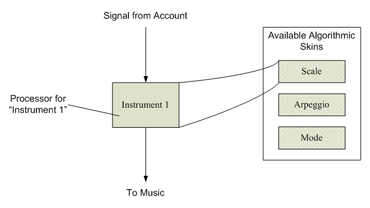
\includegraphics[scale=0.75]{Mapping_04}
\caption{Showing how a processor can be skinned from a selection of choices.}
\label{fig:map04}
\end{figure}

\noindent The skins themselves have a number of field values which can be set to make the processor's sound differ from other processors with the same skin (figure: \ref{fig:map05}).

\begin{figure}[ht]
\centering
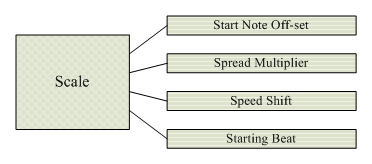
\includegraphics[scale=0.75]{Mapping_05}
\caption{Attributes of a scale, which can be set to values in order to produce a unique sound.}
\label{fig:map05}
\end{figure}

\noindent This modular approach allows for each processor to choose its skin based on the nature of the input signal. For simplicity�s sake, we will allow each processor to have only one skin applied to it. The processors work by having the signals `trigger' musical sequences by passing \textbf{threshold levels}. To understand this concept, consider the following proposition for a signal $S$ which produces musical sequence $M$:

\begin{singlespace}
\begin{formality}
$S \in \mathbbm{R}^{+}$ \\
$S \textless 0.15 \Rightarrow M = Scale$ \\
$S \textless 0.3 \Rightarrow M = Arpeggio$ \\
$S \geq 0.3 \Rightarrow M = Broken Chord$
\end{formality}
\end{singlespace}

\noindent Therefore, if we have an input signal strength of 0.14, we get a scale returned, as this signal strength is below the threshold for a scale \textit{(figure \ref{fig:sigmet01})}.

\begin{figure}[ht]
\centering
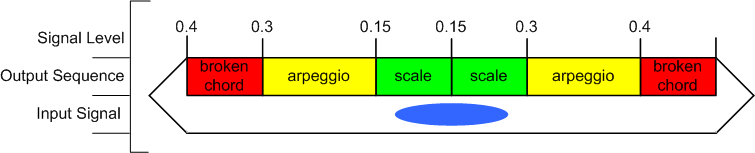
\includegraphics[scale=0.5]{sigmet01}
\caption{Diagram showing how an input signal will result in an output musical sequence by passing a threshold level. In this instance, the signal results in a scale.}
\label{fig:sigmet01}
\end{figure}

\noindent If we have a signal strength of 0.25, this \textit{is} enough to exceed the threshold for a scale, and therefore results in an arpeggio \textit{(figure \ref{fig:sigmet02})}.

\begin{figure}[ht]
\centering
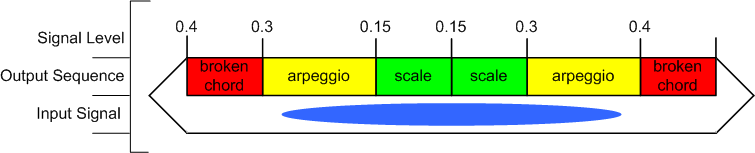
\includegraphics[scale=0.5]{sigmet02}
\caption{Diagram showing how an input signal will result in an output musical sequence by passing a threshold level. In this instance, the signal results in an arpeggio.}
\label{fig:sigmet02}
\end{figure}

\noindent If the signal strength exceeds 0.3 threshold, we get a broken chord returned \textit{(figure \ref{fig:sigmet03})}.

\begin{figure}[ht]
\centering
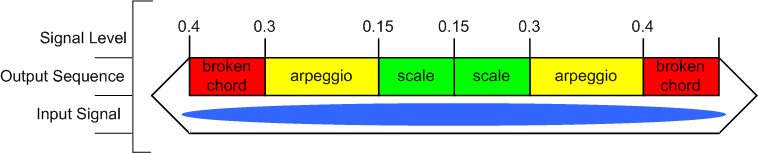
\includegraphics[scale=0.5]{sigmet03}
\caption{Diagram showing how an input signal will result in an output musical sequence by passing a threshold level. In this instance, the signal results in a broken chord.}
\label{fig:sigmet03}
\end{figure}

\section{Programming the Functions for Signal Generation}

The following functions make up the Signal Mapping implementation:
\begin{singlespace}
\begin{formality}
\texttt{prepareAccounts()}: Function to prepare the accounts and return a list of pairs. \\

\texttt{generateSignals( accounts )}: This function generates a list of signals from two accounts. The accounts are expected to be inputted as a list of pairs. \\

\texttt{orderSignals( signals, referenceSignal )}: Function to order the signals from most relevant to least relevant. \\

\texttt{signalProcessorTempo( signal )}: Tempo signal processor. \\

\texttt{getOverallKey( signal )}: Derives a key signature from a signal. \\

\texttt{signalProcessorKey( signal, referenceSignal )}: Key signal processor. Chooses the key based on the signal. As there are 12 notes in an octive (including accidentals), our output value will be between 0 and 11. \\

\texttt{signalCombinator( signals )}: This combines a set of signals into one. \\

\texttt{signalProcessorSequence( signal, referenceSignal, signalPriority )}: Produces a sequence of notes from a signal. \\

\texttt{getStartingNote( signalVariance, cutOff, signalPriority )}: Function to choose a start note within a max and min bounds. \\

\texttt{getStartingOctave( signalPriority )}: Derives a starting octave from a signal. \\

\texttt{signalProcessorScale( signal, signalVariance, signalPriority, referenceSignal )}: Produces a scale from a signal. \\

\texttt{signalProcessorArpeggio( signal, signalVariance, signalPriority, referenceSignal )}: Produces an arpeggio from a signal. \\

\texttt{signalProcessorBrokenChord( signal, signalVariance, signalPriority, referenceSignal )}: Produces a broken chord from a signal. \\

\texttt{createFullScale( octaveTemplate )}: Function to produce a complete scale for 12 octives \\

\texttt{shiftKey( octaveTemplate, keyShift )}: Function to shift the key. \\

\texttt{getKeyMap( octaveTemplate, keyShift )}: Function to produce a map of notes for a given key. \\

\texttt{mapToKey( musicalSequence, keyMap )}: Function to force a note sequence to map its self to a keyMap. \\
\end{formality}
\end{singlespace}

\noindent There is a \texttt{main()}  function which is invoked when the program is first run:

\begin{singlespace}
\begin{formality}

main( argv ): The \texttt{main( argv )} function which is invoked when the program is run. It reads the accounts, and then outputs the music.

\end{formality}
\end{singlespace}

\noindent By looking at the \texttt{main()} function, we can get a good idea of the stages that the program goes through to derive music. The pseudocode for this is given below:

\begin{singlespace}
\begin{formality}
\begin{itemize}
	\item[\textbullet] \texttt{main( argv ):}
	\begin{itemize}
		\item[\textbullet] \texttt{Read in accounts}
		\item[\textbullet] \texttt{Generate signals from accounts}
		\item[\textbullet] \texttt{Generate referenceSignal from signals}
		\item[\textbullet] \texttt{Calculate tempo from referenceSignal}
		\item[\textbullet] \texttt{Calculate key from referenceSignal}
		\item[\textbullet] \texttt{Re-order signals according to how far the deviate from referenceSignal}
		\item[\textbullet] \texttt{Initialise musicalSequences to empty list}
		\item[\textbullet] \texttt{For each signal in signals:}
		\begin{itemize}
			\item[\textbullet] \texttt{Produce a musicalSequence from signal}
			\item[\textbullet] \texttt{Append musicalSequence to musicalSequences}
		\end{itemize}
		\item[\textbullet] \texttt{If parallel approach:}
		\begin{itemize}
			\item[\textbullet] \texttt{derive overallKey from referenceSignal}
			\item[\textbullet] \texttt{for each musicalSequence in musicalSequences:}
			\begin{itemize}
				\item[\textbullet] \texttt{Shift musicalSequence into overallKey}
			\end{itemize}
			\item[\textbullet] \texttt{outputMusic = musicalSequences}
		\end{itemize}
		\item[\textbullet] \texttt{Else if sequential approach:}
		\begin{itemize}
			\item[\textbullet] \texttt{Initialise outputMusic}
			\item[\textbullet] \texttt{for each musicalSequence in musicalSequences:}
			\begin{itemize}
				\item[\textbullet] \texttt{Append musicalSequence to musicalSequences}
			\end{itemize}
		\item[\textbullet] \texttt{Send outputMusic to be played}
		\end{itemize}
	\end{itemize}
\end{itemize}
\end{formality}
\end{singlespace}

\noindent The above algorithm shows that the \texttt{main()} function dervies signals from the attributes. It then derives a reference signal (which is the same as the compound signal described earlier). This reference signal is used to calculate the tempo and overall key signature.

Next, we iterate through each signal and produce a musical sequence. Each musical sequence is appended to a list. We then consider whether we are using the sequential or parallel approach.

If we are using the parallel approach, we iterate through each music sequence and shift them into the overall key. If we are using the sequential approach, we keep each musical sequence in its current key, but we append them to each other so they play in sequence. Finally, we play (or output) the music sequence or sequences.

\section{Summary}

In this chapter we have developed a primary approach towards generating music from accounts. We have seen how we can derive signals from account attribute, and match these to musical sequences.

In the next chapter, we will attempt another approach to music generation by using biological inspiration.

\chapter{Approach 2: L-System Music Generation}

One of the biggest challenges in producing music from accounts is simply that we're using a small amount of simple data (amounts of money) to derive music, which is far more complex (sequences of notes, cords, etc). To meet this challenge, an approach is needed in which we can encourage music to ``emerge'' from something as simple as a company's balance sheet. To this end, we will turn to the field of \textbf{Biologically-Inspired Computing}.

Biologically inspired techniques tend to be good for solving complex problems with no obvious solution. Applying these techniques often leads to emergent properties, which is exactly what we're looking for. One such technique is that of the \textbf{L-System}.

In this chapter, we will look at using L-Systems to generate music from accounts. Two possible variations to achieving this will be looked at, with the most promising approach chosen for implementation and evaluation. With a working implementation, we will perform a preliminary evaluation, and then experiment with the rule generation.

\section{Definitions}

\begin{center}
\begin{singlespace}
\begin{tabular}{ l l }
\hline
\hline
\textbf{L-System}: & A Biologically-Inspired parallel re-writing system. \\ \hline
\textbf{Grammar}: & Set of symbols unique to a specific L-System. \\ \hline
\textbf{Rules}: & Part of an L-System. Specifies re-writing strategies. \\ \hline
\textbf{Axiom}: & A string of characters on which an L-System operates. \\ \hline
\hline
\end{tabular}
\end{singlespace}
\end{center}

\section{An Introduction to L-Systems}

\textbf{L-Systems} (also known as Lindenmayer Systems) were developed in 1968 by Aristid Lindenmayer. Lindenmayer was a biologist, who was trying to understand the behaviour of plant cells. During the process of his research, he developed the idea of ``an axiomatic theory of biological development''\footnote{\url{http://www.biologie.uni-hamburg.de/b-online/e28_3/lsys.html}}, which became known as the L-System. Nowadays, L-Systems have applications ranging from modeling the physical structure of plants to computer graphics. They can also be used to generate music.

L-Systems allow the re-writing of a string of characters based on a set of rules. An L-System has a \textbf{grammar}, \textbf{rules} and a \textbf{start axiom}. An L-System $G$ is formally defined as follows:

\begin{singlespace}
\begin{formality}
$G = \{ V, S, \omega, P \}$
\end{formality}
\end{singlespace}

$V$ is a set of \textbf{variables} (replaceable symbols), and $S$ is a set of \textbf{constants} (non-replaceable symbols). $P$ are the \textbf{re-writing rules} of the L-System, and $\omega$ is the \textbf{start axiom}. Rules given in $P$ will be applied to $\omega$ each time the L-System is run. 

A common example of an L-System in action is one which generates the \textbf{Fibonacci Sequence}. The Fibonacci Sequence is a sequence of numbers with very special properties. The first Fibonacci number is always 0, and the second Fibonacci number is always 1. After that, each subsequent number is defined as the sum of its two predecessors. Below is the definition of this L-System:

\begin{singlespace}
\begin{formality}
$V = \{ A, B \}$ \\
$S = \{\}$ \\
$\omega = \langle A \rangle$ \\
$P = \{ (A \rightarrow B), (B \rightarrow AB) \}$
\end{formality}
\end{singlespace}

Each time we run this L-System, we work through all the symbols in $\omega$, turning each `A'  into a `B', and each `B' into an `AB'. If we count the length of the axiom $\omega$, we get the next number in the Fibonacci Sequence:

\begin{singlespace}
\begin{formality}
start: A (axiom length = 1)\\
1st run : B (axiom length = 1)\\
2nd run : AB (axiom length = 2)\\
3rd run : BAB (axiom length = 3)\\
4th run : ABBAB (axiom length = 5)\\
5th run : BABABBAB (axiom length = 8)\\
6th run : ABBABBABABBAB (axiom length = 13)
\end{formality}
\end{singlespace}

From these simple rules, we witness a more complex property emerging. But, what happens if we define our grammar as something that can be interpreted musically?

\section{Design}
Recall that with the \textbf{Signal Mapping}, we derived signals from an account. These signals represented changes. We mapped then these signals directly to musical sequences. This time, we will instead use these signals to drive an L-System to generate music.

Two options are open for consideration. One option, is to use the accounts to generate the \textit{rules} of the L-System. The alternative is to use the accounts to generate the \textit{starting axiom}, and apply a manually crafted set of rules. Let's consider the merits of these two approaches.

\section{Variation 1: Dynamic Rule Generation}

If we decide to use the account to generate the rules, we are having to generate both the variables and the constants. Therefore, the process of generating the rules from the account must consider both musical structure (the constants in $S$) and reduction strategies (the variables in $V$). As we are generating music, we should therefore attempt to hold as much control over the constant symbols of $S$ as possible, as it is these elements that will directly translate into music.

We could be more efficient by simply using the accounts to generate the variable symbols, and define the constant symbols ourselves so that they conform to musical structures. In doing so, we may as well separate the constants and variables from one another, placing these variables in the start axiom. Doing this has the added advantage of resulting in a dynamic start axiom that will be unique for each account.

By this logic, we can conclude that Dynamic Rule Generation is \textit{not} the most efficient approach to use. But, by simplifying this idea we have derived a better approach; that of \textbf{Dynamic Axiom Generation}.

\section{Variation 2: Dynamic Axiom Generation}
Recall that instead of generating the rules from the accounts, we have chosen to manually define the rules to conform to sensible musical sequences. This way we can be assured that the L-System will produce musical sequences that will conform to what we understand to be \textit{music} rather than a chaotic collection of notes.

Now, consider that we now use the accounts to directly generate the start axiom. This will result in a unique axiom for each account, which when operated on by the L-System will produce an equally unique piece of music. The question then becomes, how can we use data in the account to generate an appropriate starting axiom?

The signal generation from the \textit{Signal Mapping} implementation presents us with a way of evaluating the health of an account, and we can build on this idea with an L-System. We can divide the potential spread of signal values into discrete grades (remember that a signal strength above \textit{1.0} indicates an increase, and below \textit{1.0} indicates a decrease). For example, let's say we try a six grade system:

\begin{singlespace}
\begin{formality}
$A > 1.25$\\
$1.25 \geq B > 1.15$\\
$1.15 \geq C > 1.05$\\
$1.05 \geq D > 0.95$\\
$0.95 \geq E > 0.85$\\
$F \leq 0.85$
\end{formality}
\end{singlespace}

By doing this, we map signal ranges to symbols. If we include these characters in the grammar of our L-System as replaceable symbols, we can define the set of variables $V$ as:

\begin{singlespace}
\begin{formality}
$V = \{ A, B, C, D, E, F \}$
\end{formality}
\end{singlespace}

\noindent An arbitrary account may therefore result in the following starting axiom\footnote{Note that although usually L-Systems uses a string to represent its axiom, I have chosen to use a \textbf{list} of \textbf{characters}. In the implementation, we will see that a list is easier to manipulate in Python.}:

\begin{singlespace}
\begin{formality}
$\omega = \langle C, D, A, B, B \rangle$
\end{formality}
\end{singlespace}

At this stage, we have successfully defined two parts of an L-System: The set $V$ of variables, and we can derive the start axiom $\omega$ from an account. The next step is to carefully choose a set of symbols which can be interpreted as music. These symbols will form the constants of $S$ in our L-System. It is at this stage that we need to decide on an appropriate grammar.

\section{Defining a Grammar}

If we look at music from the point of view of how a note in a sequence relates to its predecessor, then a note can be in one of three states; higher, lower or unchanged. We can use this to begin defining the set of variables $V$.

\begin{singlespace}
\begin{formality}
Let `u' = raise note by a tone\\
Let `d' = lower note by a tone\\
Let `s' = sustain note
\end{formality}
\end{singlespace}

Given a starting note, from these three symbols we can generate a sequence of notes. However, this grammar is quite limited, and we would like to expand it so it can better represent many more musical aspects such as chords, and key changes. To this end, we can expand the grammar with the following additions:

\begin{singlespace}
\begin{formality}
Let `/' = Raise note by two tones\\
Let `\_' = Lower note by two tones\\
Let `r' = Don't play anything (rest)\\
Let `.' = Increase overall key by a semi-tone\\
Let `,' = Decrease overall key by a semi-tone\\
Let `j' = Shift into a major key\\
Let `n' = Shift into a minor key
\end{formality}
\end{singlespace}

It would also be nice to add a harmony to complement a melody (a harmony in this case is a note played $n$ semi-tones above the note of the melody):

\begin{singlespace}
\begin{formality}
Let `+' = Turn on harmony\\
Let `-' = Turn off harmony
\end{formality}
\end{singlespace}

With this, we have a full grammar for the set $S$ of variables:

\begin{singlespace}
\begin{formality}
$S = \{ $`u', `d', `s', `/', `\_', `r', `.', `,', `j', `n' $\}$
\end{formality}
\end{singlespace}

\section{Adding Stacks to the Grammar}

In computer science, a \textbf{stack} is a primitive (yet invaluable) data structure which only allows items to be added and removed from its top. Therefore the fist item into the stack will be the last item removed, and vice-versa.

Why would we need to make use of stacks in \textit{this} L-System? Without a mechanism to jump back to earlier points in the sequence, the music would meander up and down, with no specific points to break it up. Adding a stack brings more musical structure, and allows different account attributes to affect parts of the music independently.

Many L-System implementations have built in support for the use of stacks. So, when we play the music from an axiom produced by this L-System, if we encounter a stack ``push'' symbol  (which looks like `\textbf{[}'), the program will record the current note, chord and key signature. It then continues playing the music until it reaches a stack ``pop'' symbol (which looks like `\textbf{]}'). When this happens, the program resets the note, chord and key signature to its earlier state, and continues playing the axiom.

\begin{singlespace}
\begin{formality}
Let `[' = Push current state onto stack\\
Let `]' = Pop current state from stack
\end{formality}
\end{singlespace}

\section{Interpreting the Grammar}

Turning the grammar in the axiom into music is a simple matter. Let $note$ be the current note, $tonic$ be the tonic (root note of the current key) and $scale$ be the scale (major or minor) of the current key. Let $harmony$ be whether a harmony note is being played or not.

\begin{singlespace}
\begin{formality}
$note \rightarrow \{ 21 \leq note \leq 108, note \in \mathbbm{N} \}$ \\
$tonic \rightarrow \{ 21 \leq harmony \leq 108, harmony \in \mathbbm{N} \}$ \\
$scale \rightarrow \{ major, minor \}$ \\
$harmony \rightarrow \{ true, false \}$
\end{formality}
\end{singlespace}

We initialise $note$, $tonic$, $scale$ and $harmony$ to values of our choosing, and begin to process the axiom into \textit{MIDI} values. Chords are calculated by playing a triad from the current key (notes 1, 3 and 5 of the scale)


\section{An Example in Action}

Let's look at a simple parsing example. Consider the following axiom $\omega$ generated by our L-System after a few runs:

\begin{singlespace}
\begin{formality}
$\omega = \langle$ `s', `u', `u', `d', `[', `u', `u', `u', `u', `]', `s', `d', `d', `d' $\rangle$
\end{formality}
\end{singlespace}

If we set our starting note to Middle C (MIDI value of 48), the above would transcribe the following sequence of notes:

\begin{singlespace}
\begin{formality}
48, 50, 52, 50, 52, 54, 56, 58, 50, 48, 46, 44
\end{formality}
\end{singlespace}

\section{Selecting the Rules}

With the axiom being generated by the account, the rules of the L-System must be defined manually. As we want our generated sequences to sound as musical as possible, we should ensure that our rules define short sequences with proper musical structure. To do this, we enforce some constraints when defining these short sequences.

To begin with, we can choose a \textbf{time signature}. Doing so means that we should have a consistent amount of notes in each sequence. For example, a time signature of 4 beats per bar would mean that the number of notes in each sequence must be divisible by 4.

So, we as a result of this, we might define the rules for our six-grade system as follows:

\begin{singlespace}
\begin{formality}
$( A \rightarrow j..uuuu )$\\
$( B \rightarrow [..suud] )$\\
$( C \rightarrow uuu\_uuu\_ )$\\
$( D \rightarrow ddd/ddd/ )$\\
$( E \rightarrow [,,sddu] )$\\
$( F \rightarrow n,,dddd )$
\end{formality}
\end{singlespace}

This defines some suitable musical sequences, which are appropriate for the account signal ranges they're representing. However, you will notice that after one iteration of the L-System, the axiom will be fully reduced (ie, will consist entirely of non-replaceable symbols).

To complete the rule set, we need to keep producing replaceable symbols at each iteration.  This might be done by modifying the rules to appear as follows:

\begin{singlespace}
\begin{formality}
$( A \rightarrow j..uuuuB )$\\
$( B \rightarrow [..suud]D )$\\
$( C \rightarrow uuu\_uuu\_A )$\\
$( D \rightarrow ddd/ddd/F )$\\
$( E \rightarrow [,,sddu]C )$\\
$( F \rightarrow n,,ddddE )$
\end{formality}
\end{singlespace}

The way in which the L-System produces music is often surprising, and it is not immediately obvious how to place the variables within the rules. On one hand, we want to have the music mimic the account as closely as possible. On the other hand, we want to encourage the emergence of interesting music from the L-System.

To help us choose which replaceable symbols to use, I propose that we can visualise members of $V$ occurring in $P$ as a \textbf{Finite State Machine} (FSM). In this way, when we define the set of rules $P$, we can see how the L-System will reduce the axiom $\omega$ \textit{(figure \ref{fig:fsm1})}.

\begin{figure}[ht]
\centering
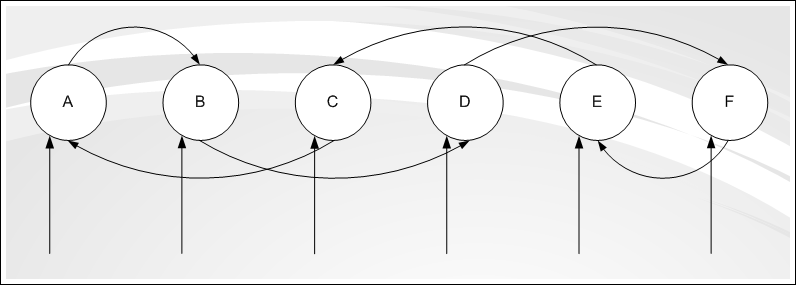
\includegraphics[scale=1.5]{fsm1}
\caption{A Finite State Machine showing a possible application of replaceable symbols within the rules of an L-System.}
\label{fig:fsm1}
\end{figure}

From \textit{figure \ref{fig:fsm1}}, we can see that our rules are probably not all that sensible. For example, $A$ reduces to a string containing $D$. This leads to more varied music being generated, but prevents a true impression being given of an account. A more sensible strategy is given in the \textit{figure \ref{fig:fsm2}}.

\begin{figure}[ht]
\centering
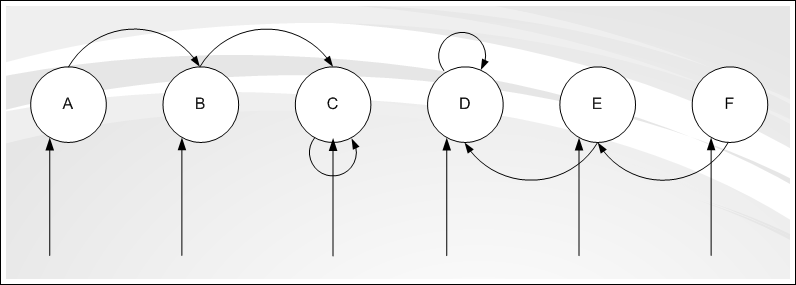
\includegraphics[scale=1.5]{fsm2}
\caption{A Finite State Machine showing a more sensible application of replaceable symbols within the rules of an L-System.}
\label{fig:fsm2}
\end{figure}

This gives us the following rules:

\begin{singlespace}
\begin{formality}
$( A \rightarrow j..uuuuB )$\\
$( B \rightarrow [..suud]C )$\\
$( C \rightarrow uuu\_uuu\_C )$\\
$( D \rightarrow ddd/ddd/D )$\\
$( E \rightarrow [,,sddu]D )$\\
$( F \rightarrow n,,ddddE )$
\end{formality}
\end{singlespace}


\section{Selecting the Number of Iterations}

With all parts of the L-System now defined, there remains one important question: How many iterations should the L-System run for?

To help answer this question, we might choose to think about the overall length of the final piece of music. If we can make a decision on roughly how many beats in total the music should play for, then we can arrange the program to keep running the L-System until the axiom length meets this requirement.

There is a good reason for taking this approach. As the listener will be paying close attention to the music, they may suffer from listening fatigue\footnote{Listening Fatigue is a lapse in concentration caused when the brain has to work hard to interpret what it's hearing. During the evaluation, testers will have to listen to lots of these musical sequences. Therefore, listening fatigue is a real concern.}, so the music should not play for too long.


\section{Programming Functions for an L-System}
The first step of implementation is to program a set of functions which can represent an L-System. By keeping as close to the formal definition as possible, and by making use of \textit{Python}'s lists and tuples, we define the following functions:

\begin{singlespace}
\begin{formality}
\texttt{getLSystem( V, S, w, P )}: Takes in the elements of an L-System, and validates them to ensure that the L-System is properly defined. If it is, it returns a tuple representing the L-System. If not, it returns an empty tuple. \\\\
\texttt{runLSystem( lSystem )}: Takes in a valid L-System tuple and applies the rules against the start axiom. It then returns the modified L-System tuple.\\\\
\texttt{getAxiom( lSystem )}: Takes in an L-System tuple, and extracts the axiom, returning it as a list of elements.
\end{formality}
\end{singlespace}

Recall that it is common for many L-Systems to make use of stacks. Therefore, this implementation implicitly includes the stack operators ``['' and ``]'' in the set of constants.

The L-System functions are kept separate from the rest of the L-System implementation, and reside in a function library \texttt{Linden.py}, which is imported into the main implementation.

\section{Programming the Axiom Generator}
The bulk of the implementation for the L-System generator resides in a new function library called \texttt{LSS.py}. Once again, we import \texttt{Settings.py} (which contains all the settings) and \texttt{Shared.py} (which contains functions shared across implementations).

For the most part, the implementation directly mimics the design strategy discussed so far in this chapter. We will begin by looking at the part of the program which generates the start axiom. Consider the following functions:

\begin{singlespace}
\begin{formality}
\texttt{generateAxiomSixGrade( signals )}: Returns a start axiom generated by splitting signal ranges into six grades.\\\\
\texttt{generateAxiomTenGrade( signals )}: Returns a start axiom generated by splitting signal ranges into ten grades.
\end{formality}
\end{singlespace}

For example, we feed the function \texttt{generateAxiomSixGrade()} the following signal list: \texttt{[1.513267626990144, 1.4732345248474281, 0.6928702010968921, 0.6676837725381415, 1.4555288461538463]}. The axiom returned might be: \texttt{['A', 'A', 'F', 'F', 'A']}. (The values which specify the grade boundaries are declared in \texttt{Settings.py}).

\section{Programming the Axiom Parser}

Interpreting the final axiom generated by the L-System is more involved than generating the start axiom. Given that we have a melody, a harmony and chords (chords are made up of \textit{three} notes), this gives us a total of \textbf{five concurrent note sequences} which are generated from the axiom. To this end, we represent each note sequence as a list of MIDI values (integers), and these lists are returned in a tuple of order 5.

The following functions are used when parsing the axiom, and are called depending on the nature of the current symbol (note that variables of set $V$ in the axiom are simply ignored during parsing):

\begin{singlespace}
\begin{formality}
\texttt{appendHarmony( outputMusicHarmony, currentNote, harmonize, harmonyKey, keyMap )}: Takes in a list of harmony notes (\texttt{outputHarmony}) and uses the other parameters to append the harmony note to this list. It then returns it.\\\\
\texttt{getDefaultKeyMap( keyMap )}: Returns a \texttt{keyMap} which is used by functions such as \texttt{pitchUp()} to determine where adjacent notes are in the scale.\\\\
\texttt{pitchUp( note, keyMap )}: Increases \texttt{note} to the next note above in the scale.\\\\
\texttt{pitchDown( note, keyMap )}: Decreases \texttt{note} to the next note below in the scale.\\\\
\texttt{doublePitchUp( note, keyMap )}: Increases \texttt{note} two note up in the scale.\\\\
\texttt{doublePitchDown( note, keyMap )}: Decreases \texttt{note} two note up in the scale.\\\\
\texttt{keyShiftUp( keyMap, shiftDistance, note )}: Shifts \texttt{keyMap} up by \texttt{shiftDistance}. Returns a shifted \texttt{keyMap} and a shifted \texttt{note} as a pair.\\\\
\texttt{keyShiftDown( keyMap, shiftDistance, note )}: Shifts \texttt{keyMap} down by \texttt{shiftDistance}. Returns a shifted \texttt{keyMap} and a shifted \texttt{note} as a pair.\\\\
\texttt{getChord( keyMap )}: Returns a tuple consisting of the 1st, 3rd and 5th note of the scale.\\\\
\texttt{chordComparison( currentChord, lastChord )}: Compares two chords. If the two chords are the same, it sustains the chord. Otehrwise, it plays the new chord. This is used to stop the chord being re-played each beat.\\\\
\texttt{keySwitchMinor( keyMap )}: Shifts \texttt{keyMap} into a minor key.\\\\
\texttt{keySwitchMajor( keyMap )}: Shifts \texttt{keyMap} into a major key.
\end{formality}
\end{singlespace}

\noindent With these functions now written and successfully tested for robustness, we have two more functions to define which complete the program:

\begin{singlespace}
\begin{formality}
\texttt{produceMusic( axiom, startNote, keyMap )}: Takes in an axiom, a start note and a key signature. Returns a tuple with lists of MIDI values.\\\\
\texttt{main( argv )}: The main() function which is invoked when the program is run. It reads the accounts, generates and runs the L-System, calls \texttt{produceMusic()} and then outputs the music.
\end{formality}
\end{singlespace}

As these two functions are so important, their pseudocode is given below. Firstly we'll look at \texttt{produceMusic()}:

\begin{singlespace}
\begin{formality}
\begin{itemize}
	\item[\textbullet] \texttt{produceMusic( axiom, startNote, keyMap ):}
	\begin{itemize}
		\item[\textbullet] \texttt{Initialise currentNote = startNote}
		\item[\textbullet] \texttt{Initialise currentChord = NULL}
		\item[\textbullet] \texttt{Initialise outputMusic = $\langle$$\rangle$}
		\item[\textbullet] \texttt{Initialise harmony = NULL}
		\item[\textbullet] \texttt{Initialise harmonize = false}
		\item[\textbullet] \texttt{Initialise noteStack = $\langle$$\rangle$}
		\item[\textbullet] \texttt{For each character in axiom:}
		\begin{itemize}
			\item[\textbullet] \texttt{if $c$ == `u' then increase currentNote by 1 tone}
			\item[\textbullet] \texttt{if $c$ == `d' then decrease currentNote by 1 tone}
			\item[\textbullet] \texttt{if $c$ == `/' then increase currentNote by 2 tones}
			\item[\textbullet] \texttt{if $c$ == `\_' then decrease currentNote by 2 tones}
			\item[\textbullet] \texttt{if $c$ == `s' then sustain currentNote}
			\item[\textbullet] \texttt{if $c$ == `r' then currentNote = NULL}
			\item[\textbullet] \texttt{if $c$ == `.' then increase keyMap's tonic by 1}
			\item[\textbullet] \texttt{if $c$ == `,' then decrease keyMap's tonic by 1}
			\item[\textbullet] \texttt{if $c$ == `j' then shift keyMap into a major key}
			\item[\textbullet] \texttt{if $c$ == `n' then shift keyMap into a minor key}
			\item[\textbullet] \texttt{if $c$ == `+' then harmonize = true}
			\item[\textbullet] \texttt{if $c$ == `-' then harmonize = false}
			\item[\textbullet] \texttt{if $c$ == `[' then push currentNote, harmonize \& keyMap onto noteStack}
			\item[\textbullet] \texttt{if $c$ == `]' then pop currentNote, harmonize \& keyMap from noteStack}
		\end{itemize}
		\item[\textbullet] \texttt{currentChord = 1st, 3rd and 5th note of keyMap}
		\item[\textbullet] \texttt{if harmonize == true \&\& keyMap in major then harmony = currentNote + 4 semitones}
		\item[\textbullet] \texttt{else if harmonize == true \&\& keyMap in minor then harmony = currentNote + 3 semitones}
		\item[\textbullet] \texttt{else harmony = NULL}
		\item[\textbullet] \texttt{Append currentNote, harmony \& currentChord to outputMusic}
	\end{itemize}
	\item[\textbullet] \texttt{return outputMusic}
\end{itemize}
\end{formality}
\end{singlespace}

From the above pseudocode, we can see that the algorithm begins with a starting note, and a key signature (consisting of a tonic and scale). Then, for each character in the axiom, it makes adjustments to these attributes.

For each axiom processed, we count that as one beat of the bar. Therefore, after processing each character, it records the current state of the attributes to \texttt{outputMusic}.

The \texttt{main()} function works in a similar fashion to the Signal Mapping's implementation. Here is the pseudocode:

\begin{singlespace}
\begin{formality}
\begin{itemize}
	\item[\textbullet] \texttt{main( argv ):}
	\begin{itemize}
		\item[\textbullet] \texttt{Read in accounts}
		\item[\textbullet] \texttt{Generate signals from accounts}
		\item[\textbullet] \texttt{Generate compoundSignal from signals}
		\item[\textbullet] \texttt{if compoundSignal > 1.0 then keyMap in major}
		\item[\textbullet] \texttt{else keyMap in minor}
		\item[\textbullet] \texttt{l\_system = new L-System generated from specification in Settings.py}
		\item[\textbullet] \texttt{run l\_system until axiom length $\geq$ minimum specified in Settings.py}
		\item[\textbullet] \texttt{outputMusic = produceMusic( l\_system.axiom )}
		\item[\textbullet] \texttt{Send outputMusic to be played}
	\end{itemize}
\end{itemize}
\end{formality}
\end{singlespace}

\section{Preliminary Evaluation}

A preliminary evaluation of this approach was performed consisting of just a few testers. The objective was to try out several rule sets and decide which one would be used in the full evaluation.

The discovery was that the sequences produced were much more musical (more complex) than the Signal Mapping approach. From this, we can formulate a testable hypothesis; That the more complex the music, the harder it will be to accurately determine the true nature of the account.\textit{(figure \ref{fig:slider1})}.

In arriving at this conclusion, we would use a simple rule set (such as the ones given in this chapter) for the coming evaluation.

\begin{figure}[ht]
\centering
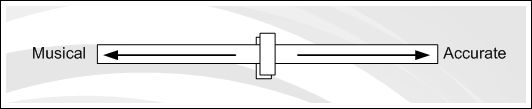
\includegraphics[scale=1.5]{slider1}
\caption{A sliding scale to show how as musicality increases, ability to accurately predict the account's health decreases. The reverse is also true.}
\label{fig:slider1}
\end{figure}

If we also take into account issues of listening fatigue, we may also conclude that the more concentration is required to analyse the music, the harder it is to predict the account's health \textit{(figure \ref{fig:slider2})}. Therefore, the maximum length of a musical sequence will be limited to under 20 seconds.

\begin{figure}[ht]
\centering
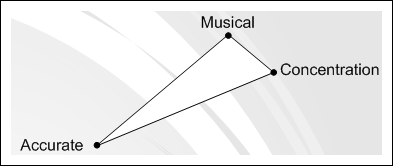
\includegraphics[scale=1.5]{slider2}
\caption{The triangle shows how increasing musicality or an increase in the need for concentration makes it more difficult to accurately predict the account.}
\label{fig:slider2}
\end{figure}


\section{Summary}

In this chapter, we have looked at L-Systems as a way of generating music from accounts. The emergent nature of L-Systems makes them well suited to an application such as music generation.

We have also seen some techniques for generating the L-System from an account, and we have settled on a way to dynamically generate the axiom using a grading system.

Finally, we also formed a hypothesis that the more complex the music, the harder it will be to determine the true nature of the account. As we will soon see, the results of the evaluation will yield some surprises.

In the next chapter, we will fully evaluate this implementation, along with the Signal Mapping approach of the previous chapter.

\chapter{Evaluation of the First Two Implementations}

\begin{quote}
``Inspiration may be a form of super-consciousness, or perhaps of sub consciousness, I wouldn't know. But I am sure it is the antithesis of self-consciousness.'' �- Aaron Copland
\end{quote}

\noindent In this chapter, we will evaluate the Mapping and L-System implementation with a carefully considered strategy. This strategy will place special emphasis on the main problem posed by this project; that \textbf{music is subjective}.

\section{How Can an Objective Evaluation be made of a Subjective Concept?}

Recall that we looked briefly at the concepts of \textbf{music cognition}. From these concepts, we understood that sound is ``processed'' into music by a human based on their personal experience. In other words; music is subjective.

How can we describe aspects of an account that will present themselves through the generated music? How can we ensure that these aspects are described in a way that \textit{both} represent the aspects of the account \textit{and} corresponding aspects of the music that relate to the account?

To help answer this, a simple analysis of publications such as \textit{The Financial Times} is called for. A browse through will reveal a surplus of buzz-words which can be used to describe aspects of an account (figure: \ref{fig:wordcloud}). An accountant who is looking at an accountant will develop an overall impression of an account. They can then describe it to a novice using a selection of these words. A novice, with little understanding of accountancy, can then understand the overall state of the account. These buzz-words are both accessible to an expert accountant, and a novice.

\begin{figure}[ht]
\centering
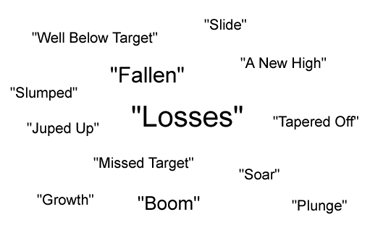
\includegraphics[scale=0.75]{word_cloud}
\caption{This word cloud shows how frequently some buzzwords occur in financial articles. The larger the font size, the greater the word's frequency.}
\label{fig:wordcloud}
\end{figure}

As an example, consider a company with vastly increasing debts and vastly decreasing profit. We give this company's balance sheet to an expert to analyse. Their experience allows them to perceive the dire state of this company, and choose the word ``plunge'' to describe the company's state.

Now consider that we generate music from this account using one of the strategies developed in previous chapters. This music is played to someone who has not seen the balance sheet. What they might hear is a lot of descending scales in a minor key quickly moving downwards. They may well also choose to describe this as a ``plunge''. It is this \textbf{synchronisation} of descriptions that we are looking for when we evaluate the approaches.

Therefore it is these buzz-words that will be the key to bridging the descriptive gap between the accounts and the generated music.

\section{Human Factors}

In the previous chapter, we briefly mentioned the issue of \textbf{listening fatigue}. If the tester's concentration lapses during the testing, they will have the opportunity to play a sequence again. They will also have the opportunity to take breaks during the testing process. Additionally, sequence length are limited to a maximum of 20 seconds, and the whole testing process is intended to take no longer than 20 minutes.

\section{Preparation of Test Data}

Fifteen accounts were sent to the expert to be evaluated. From these, \textbf{six were chosen}. Of these, \textbf{Three} were selected which displayed mostly \textbf{desirable aspects} (good investment proposition), and \textbf{Three} were selected which displayed mostly \textbf{undesirable aspects} (bad investment proposition).

From the approaches, \textbf{four methods} of generating music were chosen. From the \textbf{Signal Mapping} approach, music was generated both in \textbf{sequence} and in \textbf{parallel}. And, from the \textbf{L-System} approach, music was generated firstly with \textbf{strings and piano} and then with \textbf{piano only in staccato}.

This results in a total of 24 generated musical sequences which were prepared for evaluation. These musical sequences were then \textbf{shuffled randomly}.

\section{Designing an Evaluation Strategy}

With most testing strategies, a baseline is needed which can be used as a fixed point for comparing data. For this, an accountant was asked to analyse 16 accounts (A sample of the questionnaire that the accountant received can be seen in \textit{figures \ref{fig:qa1}, \ref{fig:qa2} and \ref{fig:qa3}} of the appendix).

The accountant was asked to choose a selection of terms to describe the \textit{account}, and were also asked to state whether they would invest in the company based on what they'd seen (they could select `yes', `no' or `unsure').

\begin{figure}[ht]
\centering
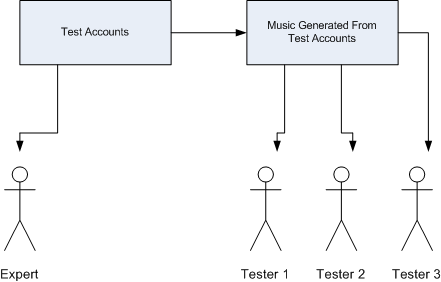
\includegraphics[scale=0.7]{testing.png}
\caption{A diagram showing how the evaluation process is organised.}
\label{fig:testing.png}
\end{figure}

For the testers who would be listening to the music, they will have to choose a selection of terms to describe the \textit{music}, and also make an assessment as to whether they'd invest in the company or not (A sample of the questionnaire that the testers received can be seen in \textit{figures \ref{fig:qt1} and \ref{fig:qt2}} of the appendix). The testers were all students, but from a variety of academic disciplines.

The testers were also asked to assess the `musicality' of each music sequence they listened to, giving it a rating from 1 (not musical) to 5 (very musical).

The motivation behind this strategy as that both the accountant and testers are using the same terminology to evaluate the account.

The tester was provided with the following information before testing:

\begin{singlespace}
\begin{formality}
\begin{enumerate}
\item That the music is generated from company accounts by a computer.
\item That the music is intended to reflect the state of the account.
\item That the test has no `right' or `wrong' answers.
\end{enumerate}
\end{formality}
\end{singlespace}

\noindent The testers are \textit{not} aware of the following details:

\begin{singlespace}
\begin{formality}
\begin{enumerate}
\item That the music they are listening to is generated by four different methods
\item That there is actually only a total of six accounts, not twenty-four.
\end{enumerate}
\end{formality}
\end{singlespace}

\noindent The testers are left to assume that each piece of music represents a unique account (although the more perceptive testers may well have guessed that this was not the case) The above approach attempts to counter the issue of subjectivity by doing the following:

\begin{singlespace}
\begin{enumerate}
\item Taking a baseline analysis of the account by asking the opinion of an `expert' (an accountant). This baseline will be used as the origin for comparison with other test results.
\item The tester is intended to be kept in the dark that they are listening to each account four times over.
\item The random ordering help remove any bias if the tester does suspect that they�re going over the same accounts twice.
\item The random ordering help evenly disperse statistical noise caused by listening fatigue.
\end{enumerate}
\end{singlespace}

\section{Results Analysis}

Before beginning analysis of the results, we need to clarify the terms used in this section:

\begin{center}
\begin{singlespace}
\begin{tabular}{ l l }
\hline
\hline
\textbf{The Expert} & A practicing chartered accountant who analysed the accounts. \\ \hline
\textbf{The Tester} & One of several individuals who evaluated the musical output. \\ \hline
\textbf{Output type} & One of the four music generation strategies. \\ \hline
\hline
\end{tabular}
\end{singlespace}
\end{center}

\begin{figure}[ht]
\centering
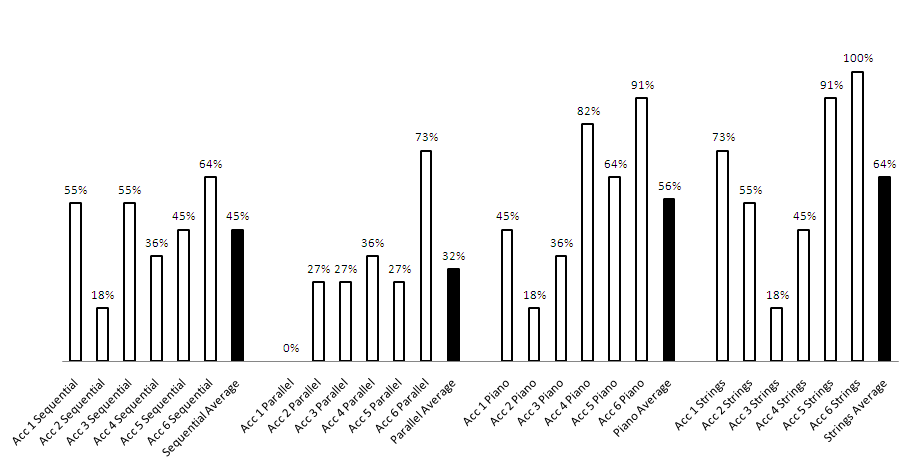
\includegraphics[scale=0.5]{agreegraph}
\caption{A graph showing the average amount that testers agreed with the expert's decision whether to invest in an account, not invest in an account or to remain undecided. (note that `strings' and `piano' are L-System generated sequences)}
\label{fig:agreegraph}
\end{figure}

\begin{figure}[ht]
\centering
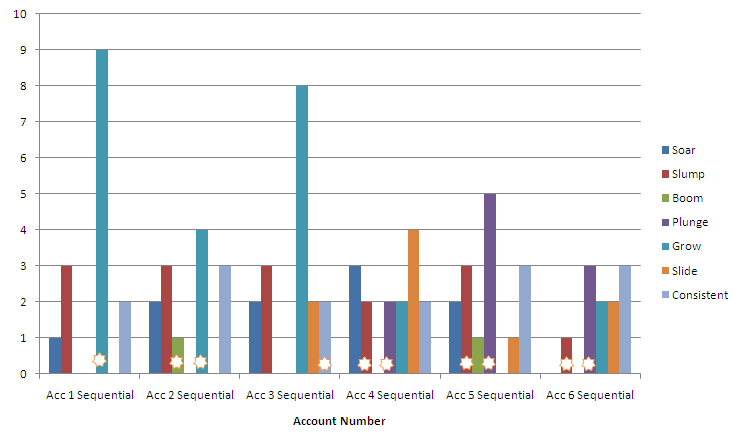
\includegraphics[scale=0.6]{agreegraphseq}
\caption{A graph showing how many times testers selected buzzwords for each account in the Signal Mapping Sequential output. A star designates that this option was selected by the expert.}
\label{fig:agreegraphseq}
\end{figure}

\begin{figure}[ht]
\centering
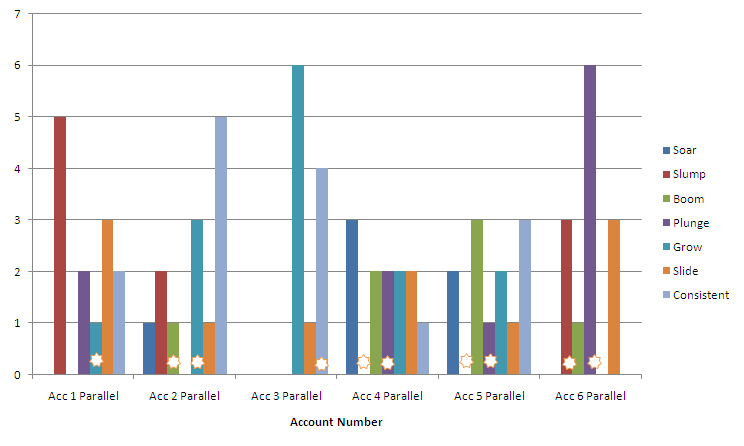
\includegraphics[scale=0.6]{agreegraphpar}
\caption{A graph showing how many times testers selected buzzwords for each account in the Signal Mapping Parallel output. A star designates that this option was selected by the expert.}
\label{fig:agreegraphpar}
\end{figure}

\begin{figure}[ht]
\centering
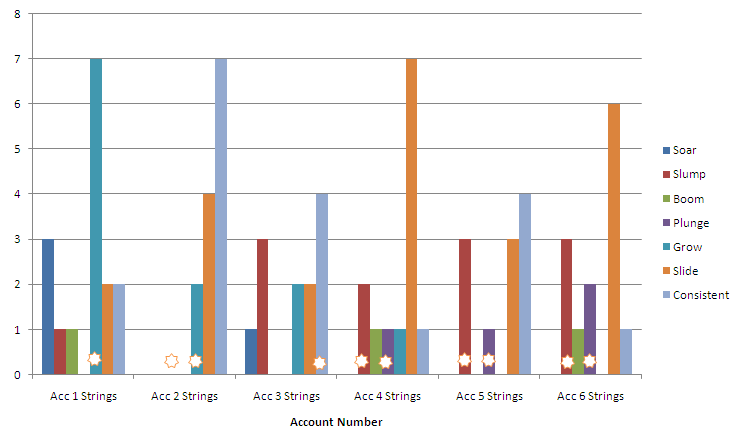
\includegraphics[scale=0.6]{agreegraphstrings}
\caption{A graph showing how many times testers selected buzzwords for each account in the L-System Strings output. A star designates that this option was selected by the expert.}
\label{fig:agreegraphstrings}
\end{figure}

\begin{figure}[ht]
\centering
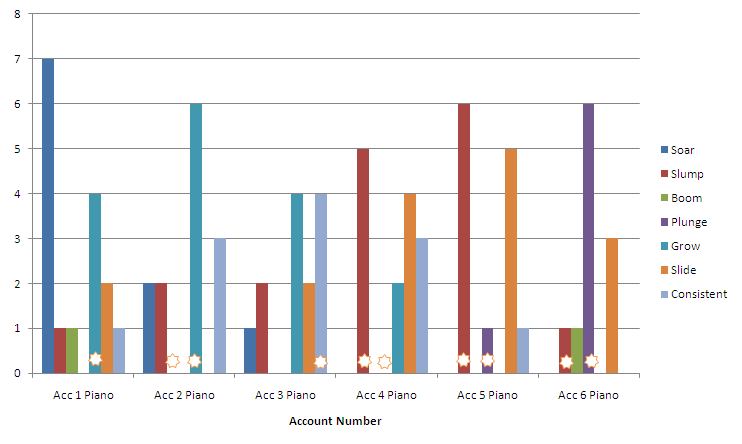
\includegraphics[scale=0.6]{agreegraphpiano}
\caption{A graph showing how many times testers selected buzzwords for each account in the L-System Strings output. A star designates that this option was selected by the expert.}
\label{fig:agreegraphpiano}
\end{figure}

\noindent The challenge of the evaluation was to deduce how often the testers agreed with the investment decisions of the expert. \textit{Figure \ref{fig:agreegraph}} shows on average how much agreement there was (recall that the choice was one of \textit{three categories}: Invest, don't invest or undecided).

Looking at the averages for each of the four output types, we see that the two L-System implementations (Strings \& Piano) were more successful than the two Signal Mapping implementations (Sequential \& Parallel).

We can gain more insight if we look at how spread out the opinions of the testers were for each of the output types. This can be done by calculating their standard deviations:

\begin{singlespace}
\begin{formality}
$\sigma_{Signal\_Mapping\_Sequential} = 0.162623126$ \\
$\sigma_{Signal\_Mapping\_Parallel} = 0.235312347$ \\
$\sigma_{L-System\_Piano} = 0.305595206$ \\
$\sigma_{L-System\_Strings} = 0.30424001$
\end{formality}
\end{singlespace}

We can see that the Signal Mapping outputs show less of a spread than the L-Sytem outputs. From this we might deduce that the L-System output types were more ambiguous than the Signal Mapping output types, and therefore the tester's investment choices were more varied. Why might this be? Consider that the Signal Mapping output types were composed of simple musical sequences (scales going up, etc). These movements are clear and were easier to interpret by the testers.

The L-System output types were generated from rules, and therefore produced sequences which were not as clear cut as an ascending scale might have been. This would mean that it was more difficult to arrive at a conclusion as to the state of the account.

That said, if the L-System output types were more ambiguous than the Signal Mapping output types, then why would it be that the L-System approach would fare better? Intuitively, we might assume that simpler musical sequences would be easier to interpret. In order to solve this mystery, we need to investigate further.

Recall that we used descriptive `buzzwords' as a way of evaluating the state of an account. Both the expert and the testers selected one or more words to describe each account (or account's output sequence) based on their perception. From \textit{figures \ref{fig:agreegraphseq}, \ref{fig:agreegraphpar}, \ref{fig:agreegraphstrings} and \ref{fig:agreegraphpiano}}  we can tell how often the testers chose the same descriptive words as the expert.

What we find with the two Signal Mapping implementations is that the testers were poor at correctly picking the same buzzwords as the expert. However, with the L-System implementation, the testers were better at selecting the same word.

As \textit{both} of the two implementations are based on the same derived signals, we can trace the difference down to the L-System processing. With the Signal Mapping implementation, musical sequences are produced mechanically by performing calculations. With the L-System implementation, we have a more organic process. This process appears on the surface to produce more complex music, but in fact we would suggest that biologically-inspired techniques are better able to tune the music towards the human ear.

\begin{figure}[ht]
\centering
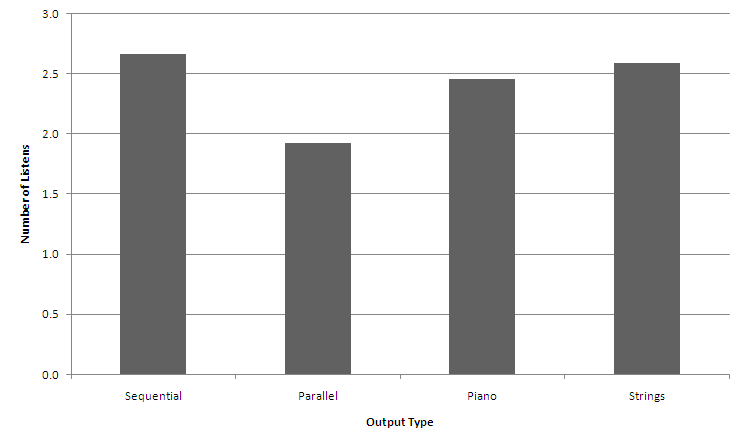
\includegraphics[scale=0.6]{numberoflistens}
\caption{A graph showing the average number of listens needed for each output type. (note that `strings' and `piano' are L-System generated sequences)}
\label{fig:numberoflistens}
\end{figure}

In terms of the average number of listens needed by each tester for each output type \textit{(figure \ref{fig:numberoflistens})}, there is an approximate correlation between the length of the sequence, and the number of listens needed \textit{(figure \ref{fig:numberoflistenscor})}. For example, a very short sequence (3 seconds) sometimes requires more listens than a longer piece (20 seconds). This is of interest to us, because the tempo reflects the amount of change in an account.

\begin{figure}[ht]
\centering
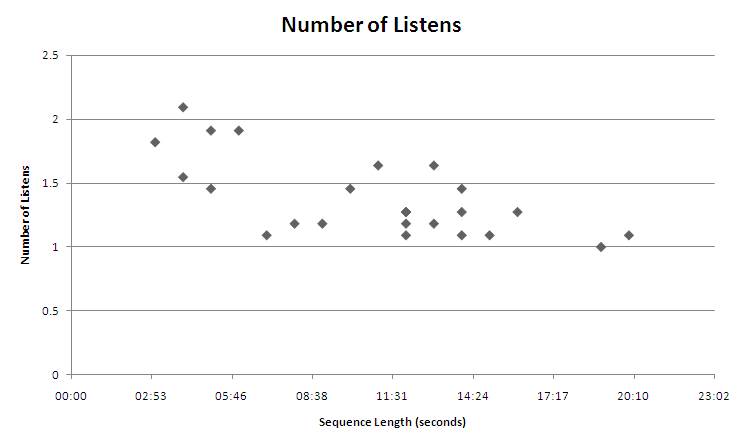
\includegraphics[scale=0.6]{numberoflistenscor}
\caption{A graph showing the correlation between the length of a musical sequence (in seconds) and the average number of listens that the tester needed.}
\label{fig:numberoflistenscor}
\end{figure}

This is also an unusual observation, because we might intuit that a short sequence would not need a further listen because it is simpler to analyse\footnote{The short-term memory model describes the way the human brain can record a small number of items in detail for up to 30 seconds. This would suggest that a shorter piece of music would be easy to hold in the mind than a longer one.}. As a concequence of this, we may wish to take into account that the tempo setting may have a side effect in the way the music was perceived by the tester.

But, what about the musicality of each approach? \textit{Figure \ref{fig:musicalityaverage}} shows how `musical' the tester considered each of the four types of output sequence to be, on a scale of 1 to 5. The two best achievers in this instance were the Sequential Signal Mapping and the Piano L-System.

\begin{figure}[ht]
\centering
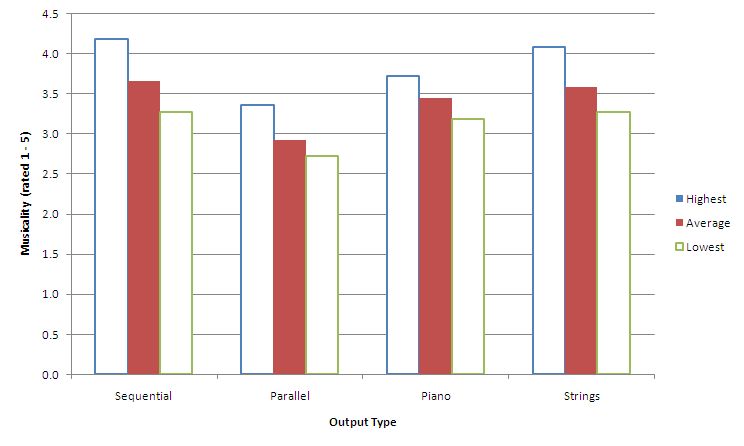
\includegraphics[scale=0.6]{musicalityaverage}
\caption{A graph showing the average spread of the musicality ratings given to each output type.}
\label{fig:musicalityaverage}
\end{figure}

Why was the prediction accuracy lower for the Signal Mapping Parallel output than it was for its Sequential counterpart? I would suggest that this is for three reasons. Primarily, we have several musical sequences playing concurrently in the Parallel output, which could make them difficult to tell apart. In the Sequential output, these sequences are played one after the other, in order of importance.

The second reason might be to do with the key shift which occurs in the Parallel output. Remember, that in order to avoid discordancy, all sequences are shifted into the same key for the Parallel output. In the Sequential output, sequences retain their own key, therefore giving them their own `flavour'.

The third reason I propose is that as the sequences are played one after another in the Sequential output, the tester was able to look at their relations to each other in a different way to having them played in parallel.  For example, key changes stand out between parts of the sequence. This perspective is lost in the Parallel output.

\section{Summary and Conclusions}

By looking at the results, we can see that \textbf{the music does to an extent represent the accounts they're generated from}. Additionally, we witness that the \textbf{L-System approach performs the best}, although both approaches do have their merits. We discovered that under ideal circumstances, testers will only correctly analyse the account from the music 64\% of the time.

\textbf{Testers considered the sequences they heard as music} (ie, have a high level of `musicality'). This is important, as one of the objectives of this project is to generate music from accounts. In this area, we can say that we have been successful.

We discovered that, paradoxically, adding an extra level of complexity to the music (via the L-System implementation) actually improves a person's ability to assess the account. This implies that the emergent properties displayed by the L-System make the nature of the accounts more clear. Perhaps it shouldn't be surprising that a biologically-inspired approach should work well when the subjects are biological!

What is really needed now is a way of formally defining the attributes in music in the same way that we can define attributes in the accounts. Achieving this would open up new avenues which would help us generate music which more closely represents the account, and it is this challenge we will attempt to meet in the next chapter.

\chapter{Approach 3: The Financial Genome}

In the previous chapter, we used a set of descriptive words to simultaneously describe features of an account and musical patterns. This technique was used to evaluate the success of the first two implementations.

In this section, we will see how these words can be used to generate a genome which represents an account. We will only go so far as to specify as way of representing this genome, and we will then define a very small genome as a way of demonstrating how this approach will work, and produce a prototype which allows some basic manipulation.

\section{Second Case Study: The Music Genome Project}

In 2006, a group of musicians developed a new way of analysing music. Their aim was to use biological inspiration to classify discrete attributes of music. They called this \textbf{The Music Genome Project}, and used this to produce the successful internet based \textit{Pandora Music} service.\footnote{http://www.pandora.com/mgp.shtml, 21st Feb 2008}

The idea they proposed was to have musicians listen to various pieces of music. They would analyse them by ear, and decide which musical elements (genes) made up the song.

Their ultimate aim was to be able to take the abstract `essences' or `moods' which make up a piece of music, and identify them as something tangible that can be used for classification. This way, when a user likes a specific song, the system can make recommendations to them based on songs with a similar genome.

\section{Notation and Definitions}

\begin{center}
\begin{singlespace}
\begin{tabular}{ l l }
\hline
\textbf{$\vert S\vert$} & The cardinality of S \\ \hline
\textbf{$\mapsto$} & Maplet (maps two elements together) \\ \hline
\textbf{Gene} & An arbitrary unit which determines a characteristic of an account or piece of music \\
\hline
\end{tabular}
\end{singlespace}
\end{center}

\section{Background}

Consider that the approach developed for the \textit{Music Genome Project} can be reversed to generate \textit{music} from \textit{accounts}. If we define a set of genomes, we can then use this as a midway point to map accounts to music. For example, each gene (we will assume a gene has only a single allele) will represent a particular part of some arbitrary music. It will also represent a specific feature in a given account. Added to this, is a set of rules which decide expression rules for sets of genes (transcription rules).

\begin{singlespace}
\begin{formality}
Let $G$ be a single gene \\
Let $A$ be an account consisting of many genes
\end{formality}
\end{singlespace}

\noindent Using the idea of using words to represent the state of an account, we can set up a financial genome for an account as follows:

\begin{singlespace}
\begin{formality}
Let $N_{f}$ be a sequence \\
Let $N_{f}$ be the genome for an account
\end{formality}
\end{singlespace}

\noindent By the same token, we can also have a musical genome given as follows:

\begin{singlespace}
\begin{formality}
Let $N_{m}$ be a sequence \\
Let $N_{m}$ be the genome for music
\end{formality}
\end{singlespace}

\noindent As $N_{f}$ and $N_{m}$ are sequences, the order is important. Take for example the relationship seen in figure \ref{fig:genes}. As elements $N_{f}$ and $N_{m}$ are mapped to specific genes, both sequences need to be specified in the order such that a gene $n$ will be expressed correctly its financial nature in $N_{f}$ and its musical nature in $N_{m}$. The genome from figure \ref{fig:genes} might therefore be sequenced as follows:

\begin{singlespace}
\begin{formality}
$F = \{0 \mapsto null, 1 \mapsto slump, 2 \mapsto soar, 3 \mapsto plunge, 4 \mapsto boom\}$ \\
$N_{a} = \{0 \mapsto null, 1 \mapsto descending, 2 \mapsto ascending\}$ \\
$N_{b} = \{0 \mapsto null, 1 \mapsto major, 2 \mapsto minor\}$ \\
$N_{c} = \{0 \mapsto null, 1 \mapsto scale, 2 \mapsto crescendo, 3 \mapsto chord\}$
\end{formality}
\end{singlespace}

\noindent The intersection of these two sequences' enumeration produces a sequence $N$, which is the general genome. $N_{f}$ and $N_{m}$ are simply expressions (phenotypes) of $\{F, N\}$.

\begin{figure}[ht]
\centering
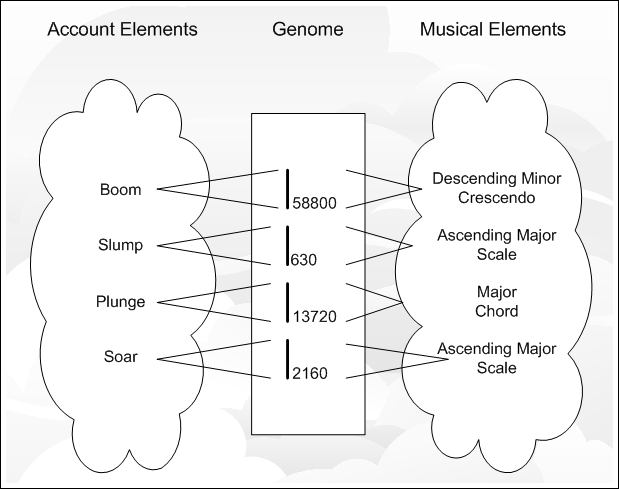
\includegraphics[scale=1.6]{genes}
\caption{Example generated from a simple genome. The genes represent both the features of an account, and also a corresponding musical feature.}
\label{fig:genes}
\end{figure}

\section{Defining Genes}

At the moment, we have a limited system where by an account feature is directly mapped to a musical feature. We can now propose that this system be extended so that an account feature can be mapped to a combination of musical elements.

The first thing that needs to be done is to define rules that take raw numbers, and reduce them to a simple \textbf{account} keyword which describes its overall state.

For example, a decrease in yearly profit from �100,000 to �90,000 is a decrease of 10\%. If we look this up in a `word table', we may find that this corresponds to the word `slump'.

We then define musical sequences in terms of words as well. In this case, I have elected to use two words to describe a musical sequence. For example, the above 10\% decrease in profit corresponds to the word `slump' which is linked to the same genome as the description `descending scale'. This fully defines a gene.

\section{Rules for Defining a Gene}

Below is a table for a specific account (and its generated music), where by each gene has a unique number: \\

\begin{center}
\begin{singlespace}
\begin{tabular}{ | l l l l l | }
\hline
\textbf{Gene \#} & \textbf{Account Wrd} & \textbf{Music Wrd 1} & \textbf{Music Wrd 2} & \textbf{Music Wrd 3} \\ \hline
58800 & Boom & Descending & Minor & Crescendo \\ \hline
630 & Slump & Ascending & Major & Scale \\ \hline
13720 & Plunge & NULL & Major & Chord \\ \hline
2160 & Soar & Ascending & Major & Scale \\
\hline
\end{tabular}
\end{singlespace}
\end{center}

\noindent The gene numbering may seem random upon first glance, but I will show in due course that there is a logical method, and that each combination of words results in a unique gene value. We will now go forward to explain how this genome was generated. We will use the following notation:

\begin{singlespace}
\begin{formality}
Let $A$ be last year�s account \\
Let $B$ be this year�s account \\
Let $F$ be a financial buzz-phrase \\
Let $W1$ be music word 1 \\
Let $W2$ be music word 2 \\
Let $W3$ be music word 3 \\
Let $G$ be a gene \\
Let $GN$ the set of all possible genes for an account
\end{formality}
\end{singlespace}

\noindent We now enumerate $F$ as follows:

\begin{center}
\begin{singlespace}
\begin{tabular}{ | l l | }
\hline
\textbf{Financial Phrase} & \textbf{Enumeration} \\ \hline
NULL & 0 \\ \hline
Slump & 1 \\ \hline
Soar & 2 \\ \hline
Plunge & 3 \\ \hline
Boom & 4 \\
\hline
\end{tabular}
\end{singlespace}
\end{center}

\noindent We also enumerate $W1$ and $W2$ as follows:

\begin{center}
\begin{singlespace}
\begin{tabular}{ | l l l | }
\hline
\textbf{Musical Word} & \textbf{Word ID} & \textbf{Enumeration} \\ \hline
NULL & W1 & 0 \\ \hline
Descending & W1 & 1 \\ \hline
Ascending & W1 & 2 \\ \hline
NULL & W2 & 0 \\ \hline
Major & W2 & 1 \\ \hline
Minor & W2 & 2 \\ \hline
NULL & W3 & 0 \\ \hline
Scale & W3 & 1 \\ \hline
Crescendo & W3 & 2 \\ \hline
Chord & W3 & 3 \\
\hline
\end{tabular}
\end{singlespace}
\end{center}

\noindent We then generate a rule table, a part of which may appear as follows:

\begin{center}
\begin{singlespace}
\begin{tabular}{ | l l | }
\hline
\textbf{ID} & \textbf{Rule} \\ \hline
1 & if $A \textgreater B$ then $W1$ = `Descending' \\ \hline
2 & if $A \leq B$ then $W1$ = `Ascending' \\ \hline
3 & if difference between $A$ and $B$ $\leq$ 10\% then $W2$ = `Scale' \\ \hline
4 & if difference between $A$ and $B$ $\textgreater$ 10\% and $\leq$ 70\% then $W2$ = `Crescendo' \\ \hline
5 & if difference between $A$ and $B$ $\textgreater$ 70\% then $W2$ = `Chord' \\ \hline
\ldots & \ldots \\
\hline
\end{tabular}
\end{singlespace}
\end{center}

\noindent From this table, $W1$ and $W2$ now have values (note, all rules must be processed until both $W1$ and $W2$ have values). We can then assign a unique identity to each gene in our genome. A \textbf{G\"odel Numbering Function} is a suitable way to achieve this, and shows how each combination of words results in a unique identifier:

\begin{singlespace}
\begin{formality}
$G = 2^{F} \cdot 3^{W_{1}} \cdot 5^{W_{2}} \cdot 7^{W_{3}}$
\end{formality}
\end{singlespace}

\noindent The reason for assigning a gene's identity in this way is so that over the processing of many different accounts, common genes can be identified. These genes will always have a unique identifier, and this feature will become incredibly useful if we wish to implement machine learning based on human feedback to decide which genes are expressing themselves the best.

\section{Invalid Genes}

Clearly, some of these genes will be invalid. In the first case, situations such as `ascending chord' simply would not make sense. You will notice that there are several $NULL$ values which can be attributed to a gene. These exist simply so that we can remove any words from a musical description without having to change the structure.\footnote{A Survey of Evolutionary Algorithms for Data Mining and Knowledge Discovery, Alex A. Freitas, section 3.1.2: \url{http://www.macs.hw.ac.uk/~dwcorne/RSR/freitas01survey.pdf}}

Also, due to the nature of the numbering function used, most values will produce genes that cannot be expressed. However, by using a rule table to detect genes, we can be assured that the genome will consist only of valid genes. Any gene enumerations not present in GN cannot be generated from an account by accident.

\section{Gene Expression}

At this point, each set of accounts has a unique genome:

\begin{singlespace}
\begin{formality}
Let $GN$ be the set of all possible genes in the genome (the genome) \\
Let $GN_{n}$ be the genome for account $n$ \\
$GN_{n} \subset GN$
\end{formality}
\end{singlespace}

\noindent Therefore, the genome for the example in \ref{fig:genes} is given as the set $GN_{example} = \{58800, 630, 13720, 2160\}$.

\section{Implementation as a Prototype}

Recall that we have a unique identifier for each gene, generated by enumerating the words and applying the enumeration to a G\"odel numbering function. Because of this, we can make use of Python's \textbf{dictionary} feature. Dictionaries store data in a similar way to lists, but instead of returning an entry via it's \textit{position} in the list, we use a key. This key will be the gene's identifier.

\noindent Here is the syntax for a gene's dictionary entry:

\begin{singlespace}
\begin{formality}
\texttt{\{ geneID: [ 'Financial Keyword', [ 'Direction', 'Key', 'SequenceType' ] ] \}}
\end{formality}
\end{singlespace}

\noindent Therefore, we might have a gene which is defined as:

\begin{singlespace}
\begin{formality}
\texttt{\{ 88200 [ 'Plunge', [ 'Ascending', 'Minor', 'Crescendo' ] ] \}}
\end{formality}
\end{singlespace}

\noindent We also need to specify which word combinations for valid genes. To do this, we define \texttt{W\_VALID} as follows:

\begin{singlespace}
\begin{formality}
\texttt{W\_VALID = [ ( ['Descending', 'Ascending'], ['Major', 'Minor'],}\\
\texttt{['Scale', 'Crescendo'] ), ( ['NULL'], ['Major', 'Minor'], ['Chord'] ) ]}
\end{formality}
\end{singlespace}

\noindent In \texttt{W\_VALID}, each tuple consists of three items. Each of these three items is a list of words. Within each tuple, the valid genes are the set produced by the cartesian product of these lists.

We then call the \texttt{getValidGenes( GN, W\_VALID )} function, which takes in our specification of valid genes, as well as the full genome (\texttt{GN}). It returns a dictionary of just the valid genes.

\section{Gene Encoding}

Encoding the genes requires a simple application of the enumeration we described above. For example, consider the following gene:

\begin{singlespace}
\begin{formality}
\texttt{\{ 1260: [ 'Soar' , [ 'Ascending', 'Major', 'Scale' ] ] }\}
\end{formality}
\end{singlespace}

\noindent Using the encoding we describe, this would result in the following list:

\begin{singlespace}
\begin{formality}
\texttt{[ 2, 2, 1, 1 ]}
\end{formality}
\end{singlespace}

\noindent It then becomes a straight forward matter to perform mutations on single genes, and evolutionary algorithms on gene sets. Seeing as each gene always results in a unique identifier, it is also straight forward to generate a G\"odel number and locate its position in the dictionary. In this way, we can determine whether the mutant is a valid gene or not.

\section{Gene Weightings}

In addition to the current setup, we assign each gene a weight based on its fitness:

\begin{singlespace}
\begin{formality}
Let $W_{n}$ be a sequence containing the weights of genes in account $n$ \\
$\vert W_{n}\vert = \vert GN_{n}\vert$ \\
Let $m$ be the weight multiplier
\end{formality}
\end{singlespace}

\noindent So, as the set $GN$ is built whilst processing the account, a sequence (represented by a list in Python) is built up. The sequence $W_{1}$ corresponding to $GN_{1}$ would be $\langle 1.0, 1.0, 1.0, 1.0 \rangle$ as each of these genes is detected only once.

Let�s say for example, that an account $GN_{2}$ has the same selection of genes as $GN_{1}$, but gene $900$ is detected twice, and gene $54000$ is detected three times. We set $m$ to a constant value of $1.5$. Each weight value is calculated as follows:

\begin{singlespace}
\begin{formality}
Let $G_{n}$ be a gene \\
Let $c$ be the number of times $G_{n}$ is detected \\
The weight of $G_{n}$ is given by $mc-1$
\end{formality}
\end{singlespace}

\noindent In the case of $GN_{2}$, this gives us $W_{2} = \langle1.0, 1.0, 1.5, 2.25\rangle$

\section{Functions of the Prototype}

Below is a full list of functions employed in the prototype:

\begin{singlespace}
\begin{formality}
\texttt{godel( a, b, c, d )}: G\"odel numbering function. \\

\texttt{displayGenome( GN )}: Function to display the genome. \\

\texttt{generateGenes( F\_SET, W1\_SET, W2\_SET, W3\_SET )}: Generate the set of all possible genes. \\

\texttt{getValidGenes( GN, W\_VALID )}: Generate the set of all valid genes (ie, those with valid musical sequences). \\

\texttt{getRandomGeneSet( n, GN\_VALID )}: Produce a random set of genes with n members. \\

\texttt{generateEncoding( gene )}: Generates an encoding for a gene. \\

\texttt{generateEncodings( genes )}: Generates encodings for a set of genes. \\

\texttt{decodeGene( encoding )}: Decodes a gene. \\

\texttt{decodeGenes( encodings )}: Decodes several genes. \\

\texttt{mutateGene( gene, validGenes )}: Performs an single-random-gene new-allele mutation given an encoding. \\

\texttt{mutateGeneSet( genes, m, validGenes )}: Performs an m-random-gene new-allele mutation on a set of genes. \\

\texttt{generateGenomeWeights( genome )}: Generate evenly distributed weights for a genome. \\

\texttt{increaseWeight( encodedGene, weights )}: Increase the weight of a gene.
\end{formality}
\end{singlespace}

\noindent The prototype operates by calling functions from within the Jython interpreter in order to perform the operations.

\section{Beyond the Prototype}

Due to time constraints, the prototype was not developed beyond its current state. The next stage would have involved plugging the genome into one of the first two implementations. A population would have been generated for an account, and its fitness evaluated in relation to the music produced. A number of experts would have been required to make this a reality.

\section{Summary}

In this, the penultimate chapter, we have seen how we can use words to describe both accounts and music. By using the cartesian product, we can produce a genome set which covers all mapping possibilities of accounts to music. The evaluation of the fitness of these genes is the domain of financial experts and musicians, and these resources lie outside the scope of this project.

Over the previous chapters, we have looked at two full implementations and one prototype. In the next chapter, we will sum up and see what conclusions have been reached from this project.








\chapter{Conclusions}

We now arrive at the end of the project, and in this final chapter we will reflect upon what we've discovered, and how future projects could continue the work.

\section{Discoveries and Achievements}

At this point, it is pertinent to ask the question ``What have we discovered from this process?''. To begin with, we discovered that it \textit{is} possible to generate music from accounts. More so, we found that by refining techniques, we could get the music to approximate the account's features, so that a listener could make a guess at the state of the account. We also discovered that a biologically-inspired approach worked much better than one which came from a purely mathematical direction.

With the conclusion of this dissertation, we have successfully managed to generate music from accounts. The evaluation implies that one of the approaches is over 60\% effective in representing the account's true nature. Recall that these were the two main aims of the project.

\section{Project Evaluation}

The purpose of this section is to clear up any ambiguities for those readers who followed this project through its first and second deliverables (The final document you are reading now would be classed as the third deliverable).

By Deliverable 2, two implementations were proposed, namely the Signal Mapping and the Financial Genome. During the course of the implementation, the L-System Music Generation idea was formulated, and showed enough promise to warrant further exploration.

In the end, a full implementation of the L-System idea was produced, and evaluated along side the Signal Mapping. Results of the evaluation showed that developing the approach was worth the time and effort put into it.

Meanwhile, the Financial Genome approach was showing signs of being too ambitious for an undergraduate dissertation. The design process continued to progress from the second deliverable, but a fully developed prototype was not able to be produced in the time available. Moreso, the ambitiousness of the idea would have made evaluating such a prototype very difficult without greater resources. In the end L-System implementation was pursued at the expense of the Financial Genome approach.

However, the Financial Genome idea was not abandoned by any means. This resulted in a greater overall quantity of work being performed than was originally proposed at the time of Deliverable 2 (three ideas instead of two). Unfortunately, the Financial Genome was not as fully developed as it was intended to be.

\section{Future Work}

The basic idea proposed of generating music from accounts is a vast one, and one with huge potential. During the course of this project, we have developed some preliminary ideas, but there is so much more work that could be done in this area. In this section, various avenues for future work are proposed.
Approximations of time scales are given with each proposal. (A \textbf{medium} timescale should be considered to be the same amount of time spent on this dissertation.) \\

\noindent \textbf{User Interface} \\

\noindent 1) Development of a user interface in Java \textit{(see appendix B, page \pageref{appendix:interfaces1})}. \textit{Time scale: short}\\

\noindent 2) Development of a web based version using a Java applet \textit{(see appendix B, page \pageref{appendix:interfaces1})}. \textit{Time scale: short} \\

\noindent 3) Ability to read accounts from websites such as \textit{Google Finance} via the use of data scraping techniques \textit{(see appendix B, page \pageref{appendix:interfaces2})}. \textit{Time scale: medium} \\

\noindent 4) Full integration into a spredsheet application, as described in Douglas Adams' book. \textit{Time scale: medium} \\

\noindent \textbf{Signal Mapping} \\

\noindent 1) In this dissertation, only the balance sheet is used to generate signals. The implementation could be expanded by also using the Income and Cash Flow statements. \textit{Time scale: medium} \\

\noindent 2) The concept of `skinning' the processors to produce different types of musical output can be applied. \textit{Time scale: medium} \\

\noindent \textbf{L-System Music Generation} \\

\noindent 1) Rule definitions: Research into how to structure the rules of the L-System so that they better reflect the account's nature. This kind of research would probably be suited to someone with a musical background. \textit{Time scale: medium to long}\\

\noindent 2) What happens if we have \textbf{longer strings} in the replacement rules? This leads to more control over the musical sequences used, but does it come at a cost? \textit{Time scale: short} \\

\noindent 3) We could use is to have additional variables in $V$ of the L-System that produce `generic' musical sequences not tied to any account features. These can be used to pad out the music, and are included simply to provide colour to the music. This will increase the musical complexity, but will it dilute the signs which point to account features? \textit{Time scale: medium} \\

\noindent 4) We could consider including more than one variable in a replacement rule. This way, the axiom reduces in a less predictable manner, leading to more emergent properties. For example, we could have a rule: $(A \rightarrow BuuC)$. \textit{Time scale: short to medium} \\

\noindent 5) A ten grade system could be applied (and indeed, the implementation already supports this). This would mean that a greater variety of music is produced, as there are more grade boundaries for signals. However, the rules for each grade need careful planning, and many more accounts are needed for testing a ten grade system than a six grade system, simply because of the greater variety of music. \textit{Time scale: short to medium} \\

\noindent 6) Each account attribute has its own set of replacement rules. This would perhaps make it easier to hear the movement of specific attributes within an account, as they could generate their own sequences. \textit{Time scale: short to medium} \\

\noindent 7) We could define musical genres, allowing the user to choose a genre of their preference before the music is generated. For example, the rules we defined in this chapter produce music which is split into four beats per bar. If we reduced this to three beats, we could set this alternative rule set up as its own `waltz' genre. \textit{Time scale: medium to long} \\

\noindent \textbf{Financial Genome} \\

\noindent 1) Research into developing a fuller financial genome. The genome given in Chapter 7 only defines a few simple characteristics. A fuller genome could lead to better music generation. \textit{Time scale: long} \\

\noindent 2) Genes can be given the ability to be dominant or recessive. They can also be developed so combining two genes produces a unique feature not found in any other configuration. \textit{Time scale: medium} \\

\noindent \textbf{General Research} \\

\noindent 1) Music cognition tells us that a person's perception of music is based on their experience. Research could be conducted into how cultural background affects the perception of the accounts when heard through the music. \textit{Time scale: long} \\

\noindent 2) There may be many other (and possibly better) approaches to generating music from accounts. Some of these could be investigated. \textit{Time scale: medium to long} \\

\noindent 3) As the generated music becomes more complex, what is the `cost' associated with this in terms of ability to accurately assess the account's true nature? \textit{Time scale: medium} \\


\section{Final Conclusion: Is There a Real-World Application for Financial Music?}

After reading through this document, the reader may conclude that whilst Financial Music is an interesting topic for research, it lacks any value as a real-world application, perhaps doomed to reside with thousands of other programming curiosities which can be found the internet.

But, if the amount of accounts that a novice can correctly analyse through the music \textit{exceeds} the amount that they can correctly analyse just from looking at the numbers, then Financial Music can serve a useful purpose. On top of this, if the music provides a \textit{quicker} way to analyse accounts than traditional methods, then we have found a real-world use for Financial Music.

For example, an investment portfolio manager could batch convert a series of accounts to music, and then listen to the tracks on their iPod whilst out jogging during their lunch break. When returning to their office, they can then choose which accounts to investigate further. Therefore, the main purpose Financial Music could serve is to help filter out the worst investment propositions. \\

\noindent Finally, It is my hope that the development of Financial Music idea will continue.





\begin{singlespace}
\chapter*{Appendices}
\addcontentsline{toc}{chapter}{Appendix}
\pagenumbering{Roman}
\section{Appendix A: Test Results}

\begin{figure}[ht]
\centering
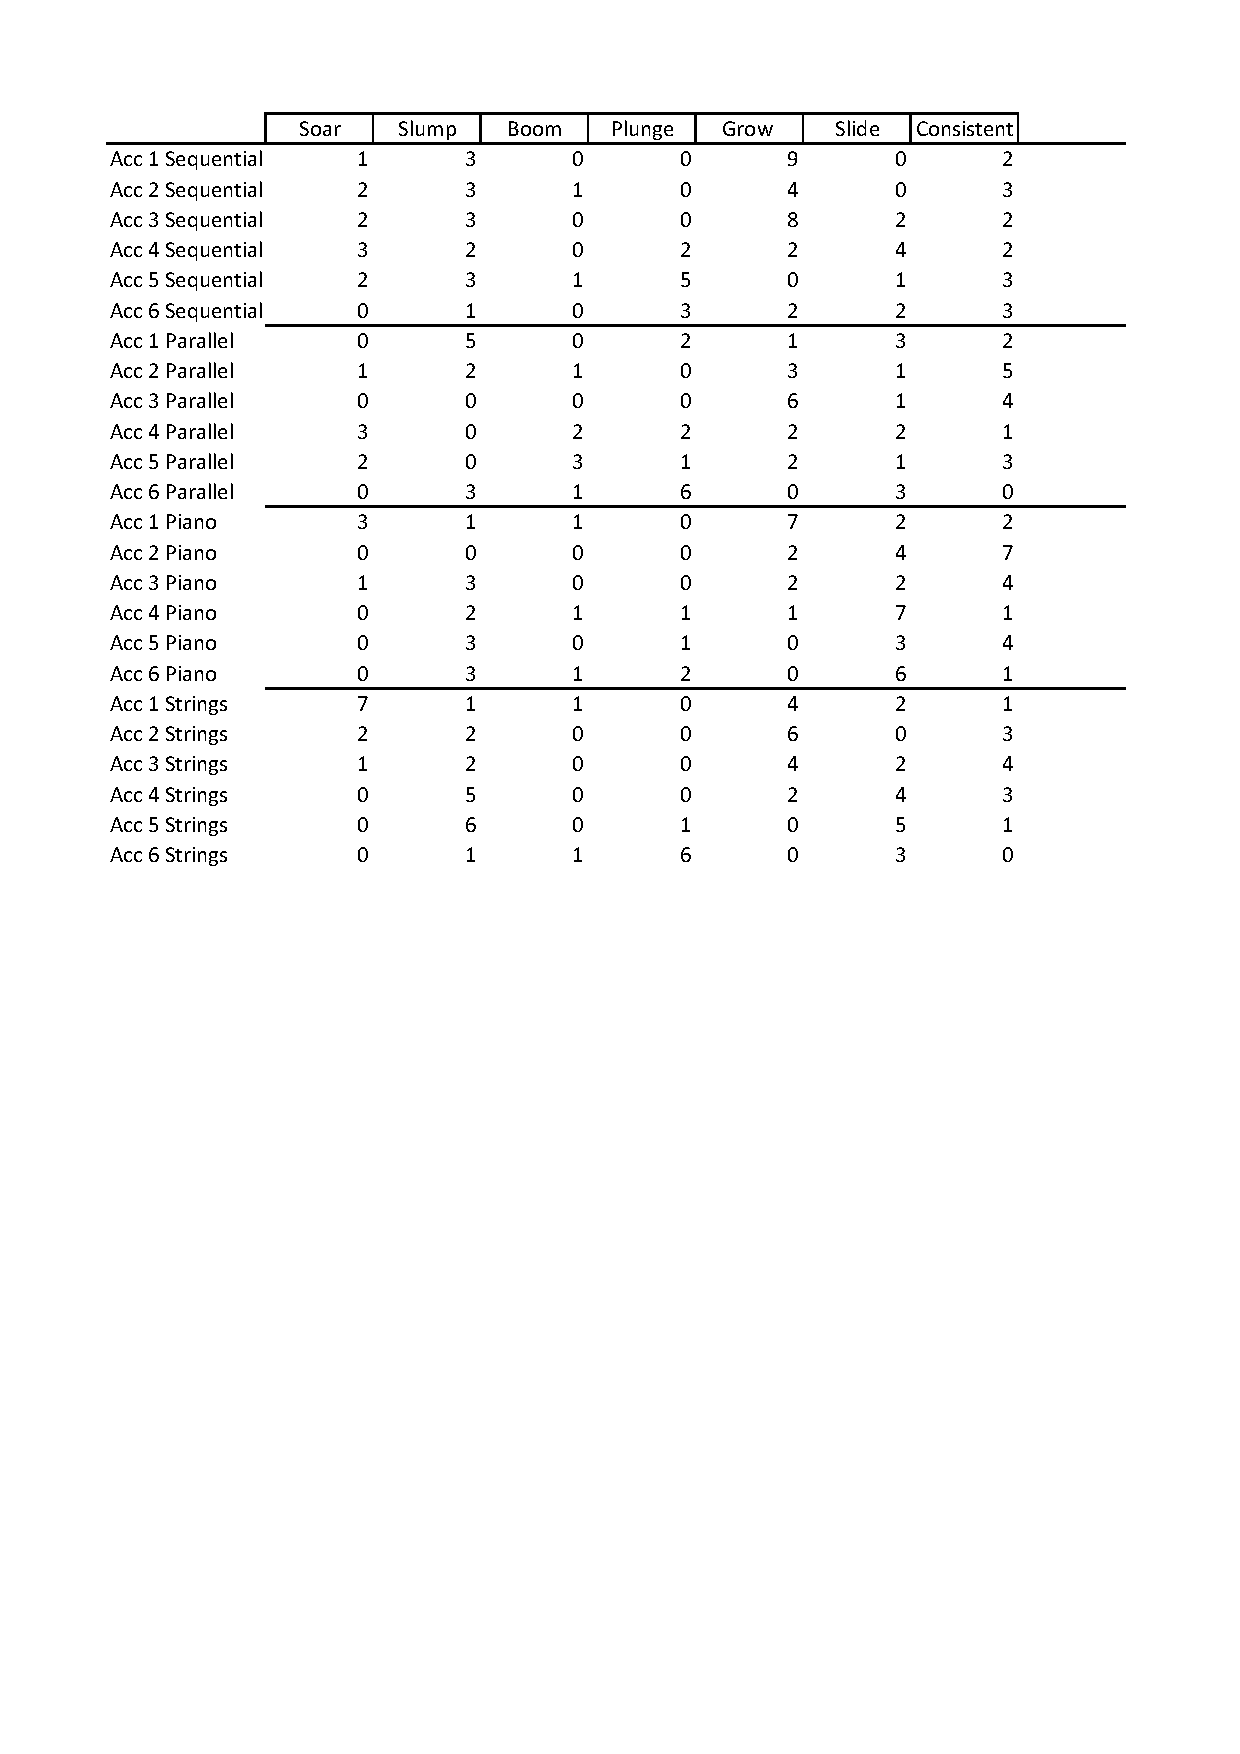
\includegraphics[scale=0.75]{results1}
\caption{Sheet 1 of the results.}
\label{fig:results}
\end{figure}

\begin{figure}[ht]
\centering
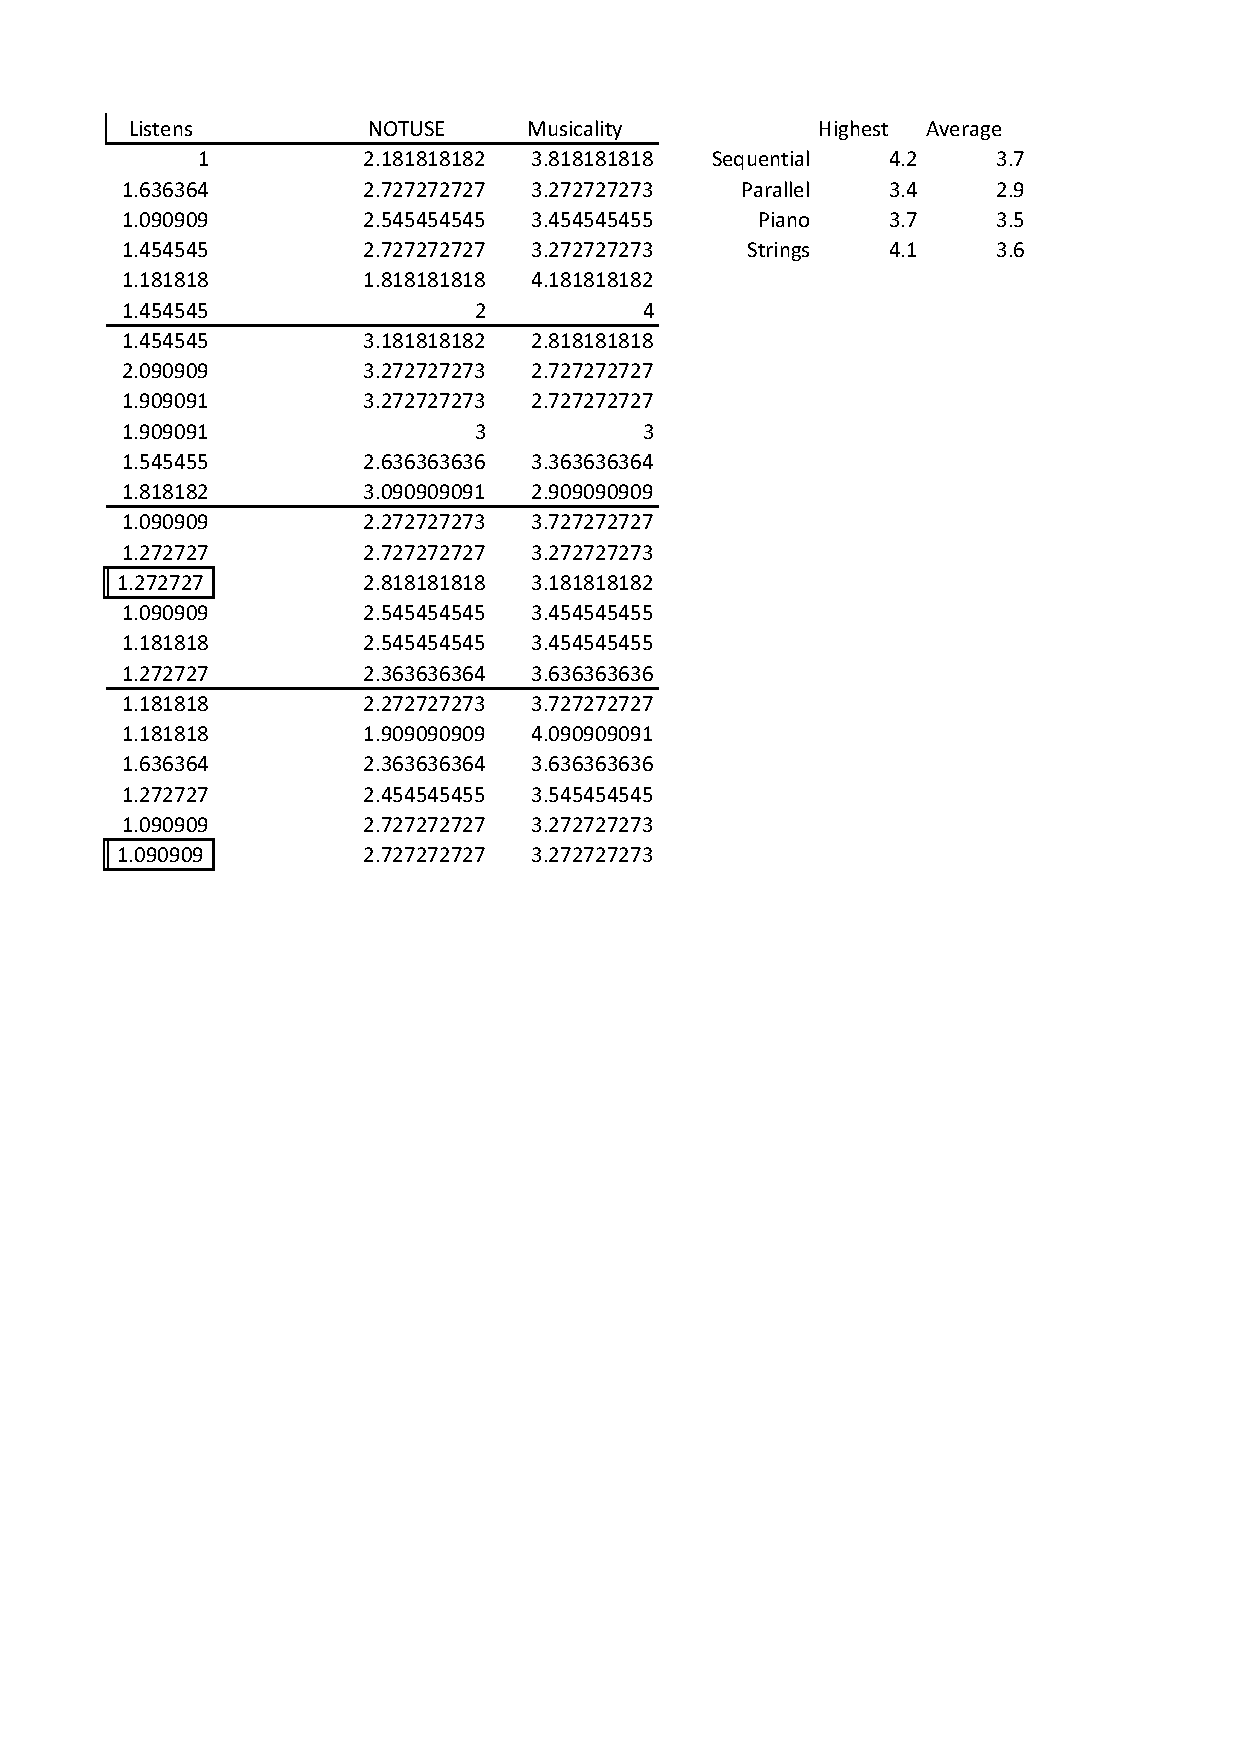
\includegraphics[scale=0.75]{results2}
\caption{Sheet 2 of the results.}
\label{fig:results}
\end{figure}

\begin{figure}[ht]
\centering
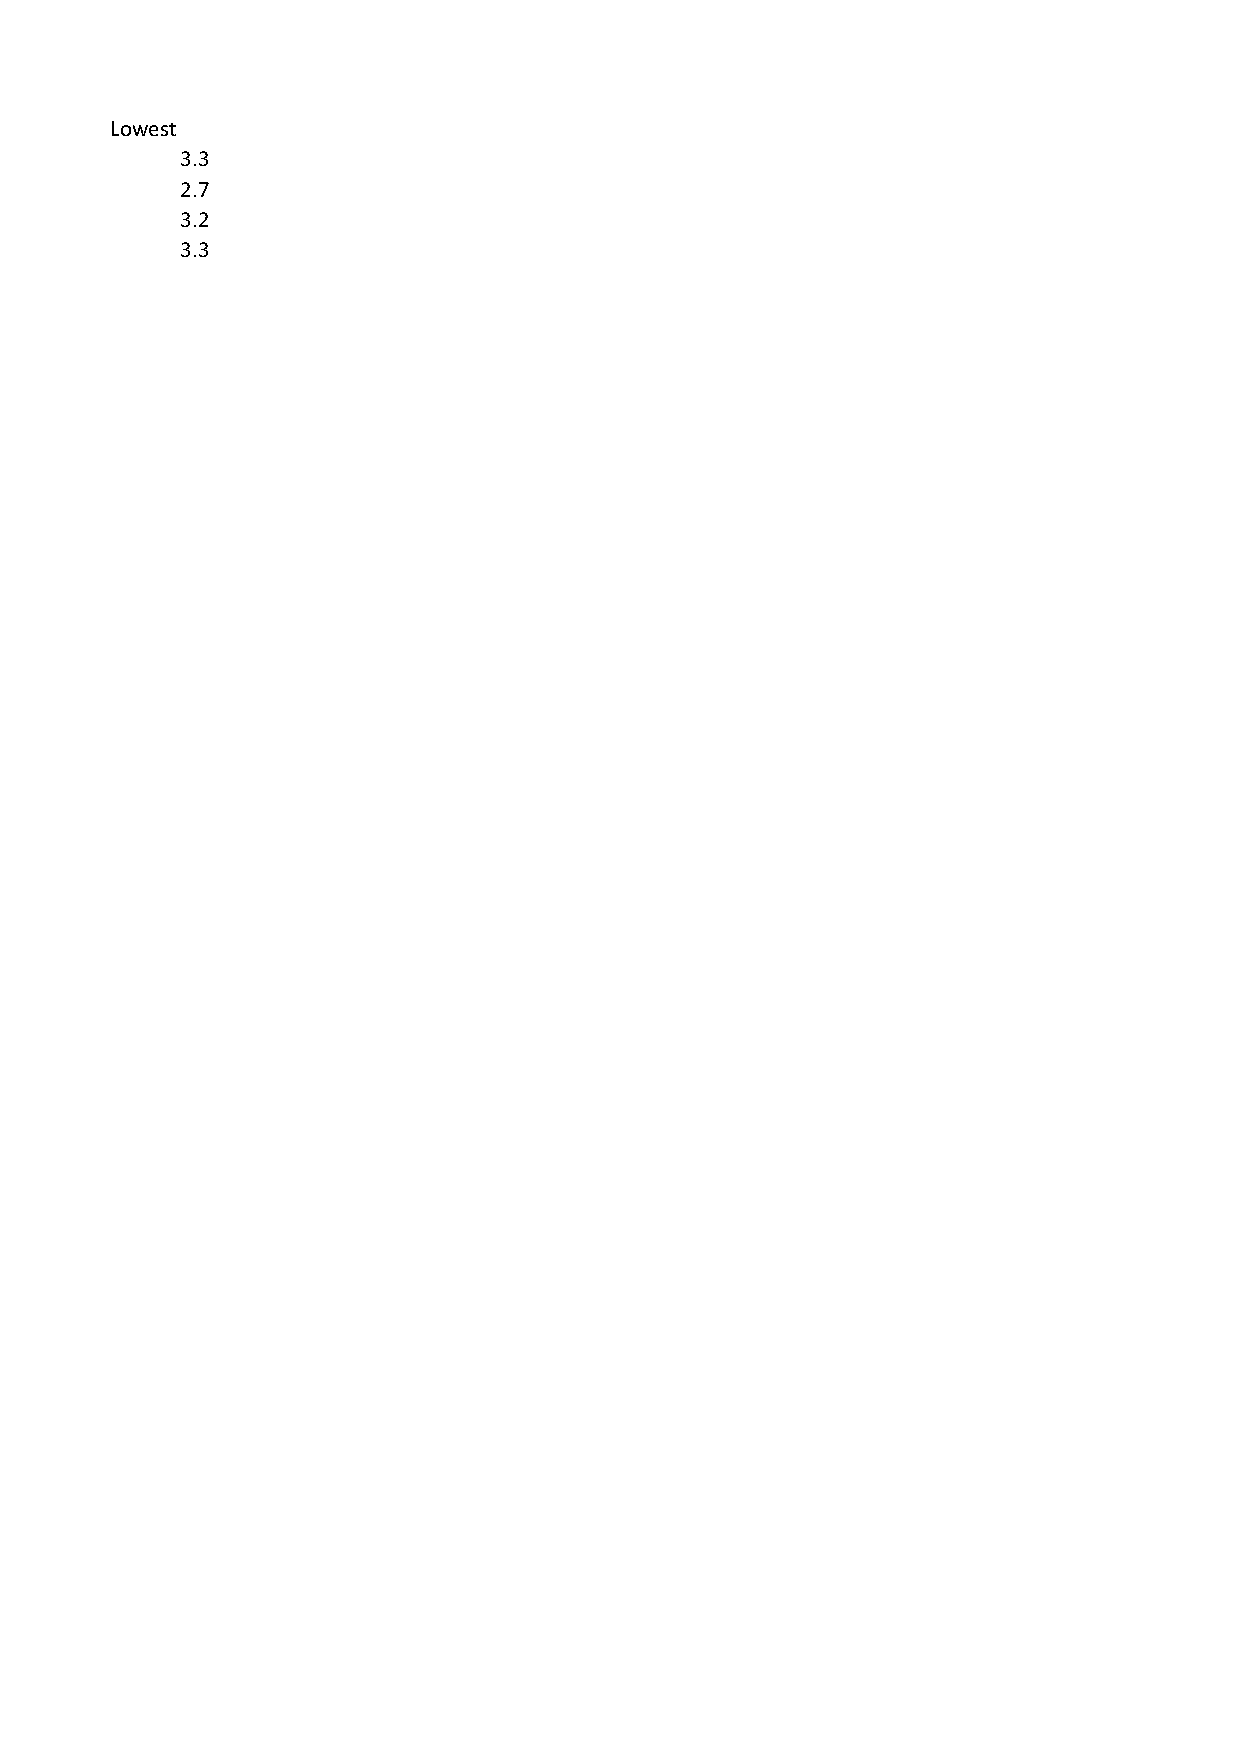
\includegraphics[scale=0.75]{results3}
\caption{Sheet 3 of the results.}
\label{fig:results}
\end{figure}
\section{Appendix B: Interfaces}

In this section, ways that account data can be imported into the Financial Music software will be explored. An ideal outcome would be that accounts can be imported directly from a website using an API, RSS feed, or other XML based protocol. However, other options will also be considered.

\subsection*{A User Interface}

\label{appendix:interfaces1}The most basic way of having the program attain account information would be to provide a simple user interface.

This interface would consist of fields which can be filled in, and a button to �submit� their contents for analysis.

This kind of interface, whilst crude, would provide a very nice way to test the software. Values could be tweaked and altered on the fly to generate music. Feedback would be instant, providing a quick mental picture of what kind of data produces what kind of music.

\subsection*{Local Sources}

My second reader suggested to me that I use \textbf{CSV} as a commonly used format for importing accounts. This would allow for the easy importing of accounts stored in spreadsheet format (figure: \ref{fig:import1}).

The system I have implemented requires that two year�s worth of accounts be set up in individual spreadsheets. These spreadsheets consist of two rows; the top row contains the headings, and the bottom row contains the numerical values.

The importing procedure runs checks to ensure that both spreadsheets have the same number of columns in the first two rows as each other, and the headings in both spreadsheets are identical. These two clauses provide reasonable assurance that the two spreadsheets are from the same template.

\begin{figure}[ht]
\centering
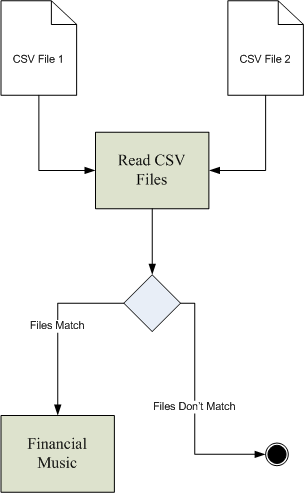
\includegraphics[scale=0.75]{import_1}
\caption{Importing CSV files into the Java application.}
\label{fig:import1}
\end{figure}

\subsection*{Internet Sources}

\label{appendix:interfaces2}The primary candidate for sourcing account information is \textbf{Google Finance}, which has recently launched a localised UK version of this service\footnote{http://finance.google.co.uk, \textit{Google Finance UK}, 01/02/2008}. Google Gadgets provides a JavaScript API for accessing data from Google Finance\footnote{http://code.google.com/apis/gadgets/docs/finance.html, \textit{Financial Gadgets}, 01/02/2008} , but due to licensing restrictions, Google have not opened up this API for use on any other platform\footnote{http://googlefinanceblog.blogspot.com/2007/10/api-gadgets-and-tabs-oh-my.html, 01/02/2008}. \textbf{Yahoo Finance} suffers from a similar restriction, and will only allow the manual generation of HTML as a �badge� that can be placed on a web log (blog) or website\footnote{http://finance.yahoo.com/badges, 01/02/2008}. It also does not provide the complete balance sheet that is needed.

\subsection*{A Workaround}

The option I'm considering is the inclusion of a JavaScript, which can be added as a \textbf{bookmarklet} (a small script or applet stored as a browser bookmark) in a web browser. This JavaScript would be able to scan a web page for specific elements (known as \textbf{data scraping}), and extract them (figure: \ref{fig:import2}). This can be done by accessing elements of the \textbf{document object model} (\textbf{DOM}). Then, the user views a company�s account on Google Finance. They then select the bookmarklet, which runs the JavaScript. The JavaScript could pass the relevant data to another page containing \textbf{Financial Music} as a Java applet\footnote{http://www.devdaily.com/java/edu/pj/pj010003/pj010003.shtml, 01/02/2008}. This would allow an account to be played with a single click. (The idea of disguising a JavaScript as a bookmark is not a new one, as it is used by Google to automate the adding of RSS feeds to Google Reader, and also by \textit{tinyurl.com} to minimise the URL of the currently viewed web page)

There are limitations to this compromise: \textit{(a)} This is all be dependent on Google not changing the setup of their web pages; otherwise the script may no longer function. \textit{(b)} The account information to be extracted is chosen by the JavaScript. Therefore, if we wish to use different account attributes, we need to alter both the JavaScript and the Java Applet to be synchronised with each other.

\begin{figure}[ht]
\centering
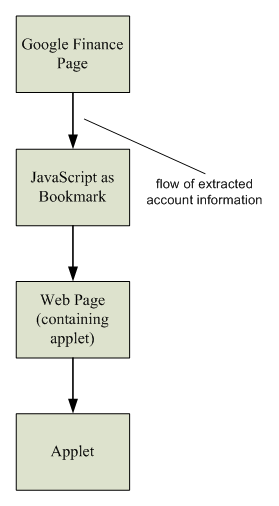
\includegraphics[scale=0.75]{import_2}
\caption{Flow of account data from Google Finance to the Java applet.}
\label{fig:import2}
\end{figure}

\subsection*{In Practice}

The reality of the situation, is that Google Finance isn't set up for easy data extraction (in an ideal situation, the relevant HTML elements would be nicely tagged with the \textit{ID} element). What we do know from looking at the HTML source, is that the value for an attribute is located directly after its label. Therefore, we need to search for the name of the account attribute we want to extract. Once this is done, the next item of data should be the value that we need to extract.

The Java applet should also have a default state, whereby if no information is passed to it via its containing web page, it will allow the user to enter account information manually.
\section{Appendix C: Evalutaion Results and Supplementary Graphs}

\begin{figure}[ht]
\centering
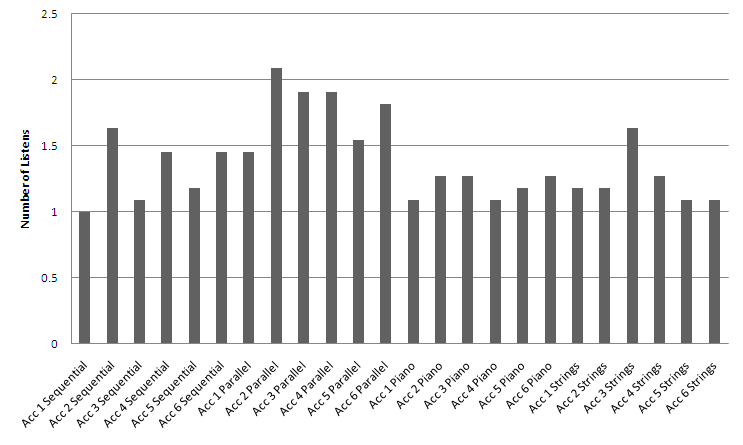
\includegraphics[scale=0.6]{numberoflistensind}
\caption{A graph showing how many times on average testers listened to each output sequence.}
\label{fig:numberoflistensind}
\end{figure}

\begin{figure}[ht]
\centering
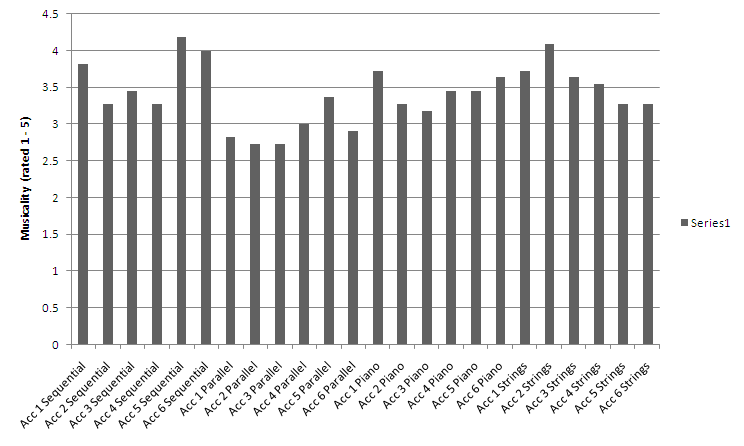
\includegraphics[scale=0.6]{musicalitydetail}
\caption{A graph showing the average musicality score between 1 and 5 that testers gave each output sequence.}
\label{fig:musicalitydetail}
\end{figure}
\section{Appendix D: Questionnaire}

In this section, I have included the questionnaires that were used by the expert and the testers to provide feedback for the evaluation. These questionnaires were provided to the testers as Microsoft Word templates. The boxes could be ticked directly, and the music sequences were embedded in the document. Once the questionnaires were filled out, they could simply be saved under a different file name, and were then archived for later analysis.

\begin{figure}[ht]
\centering
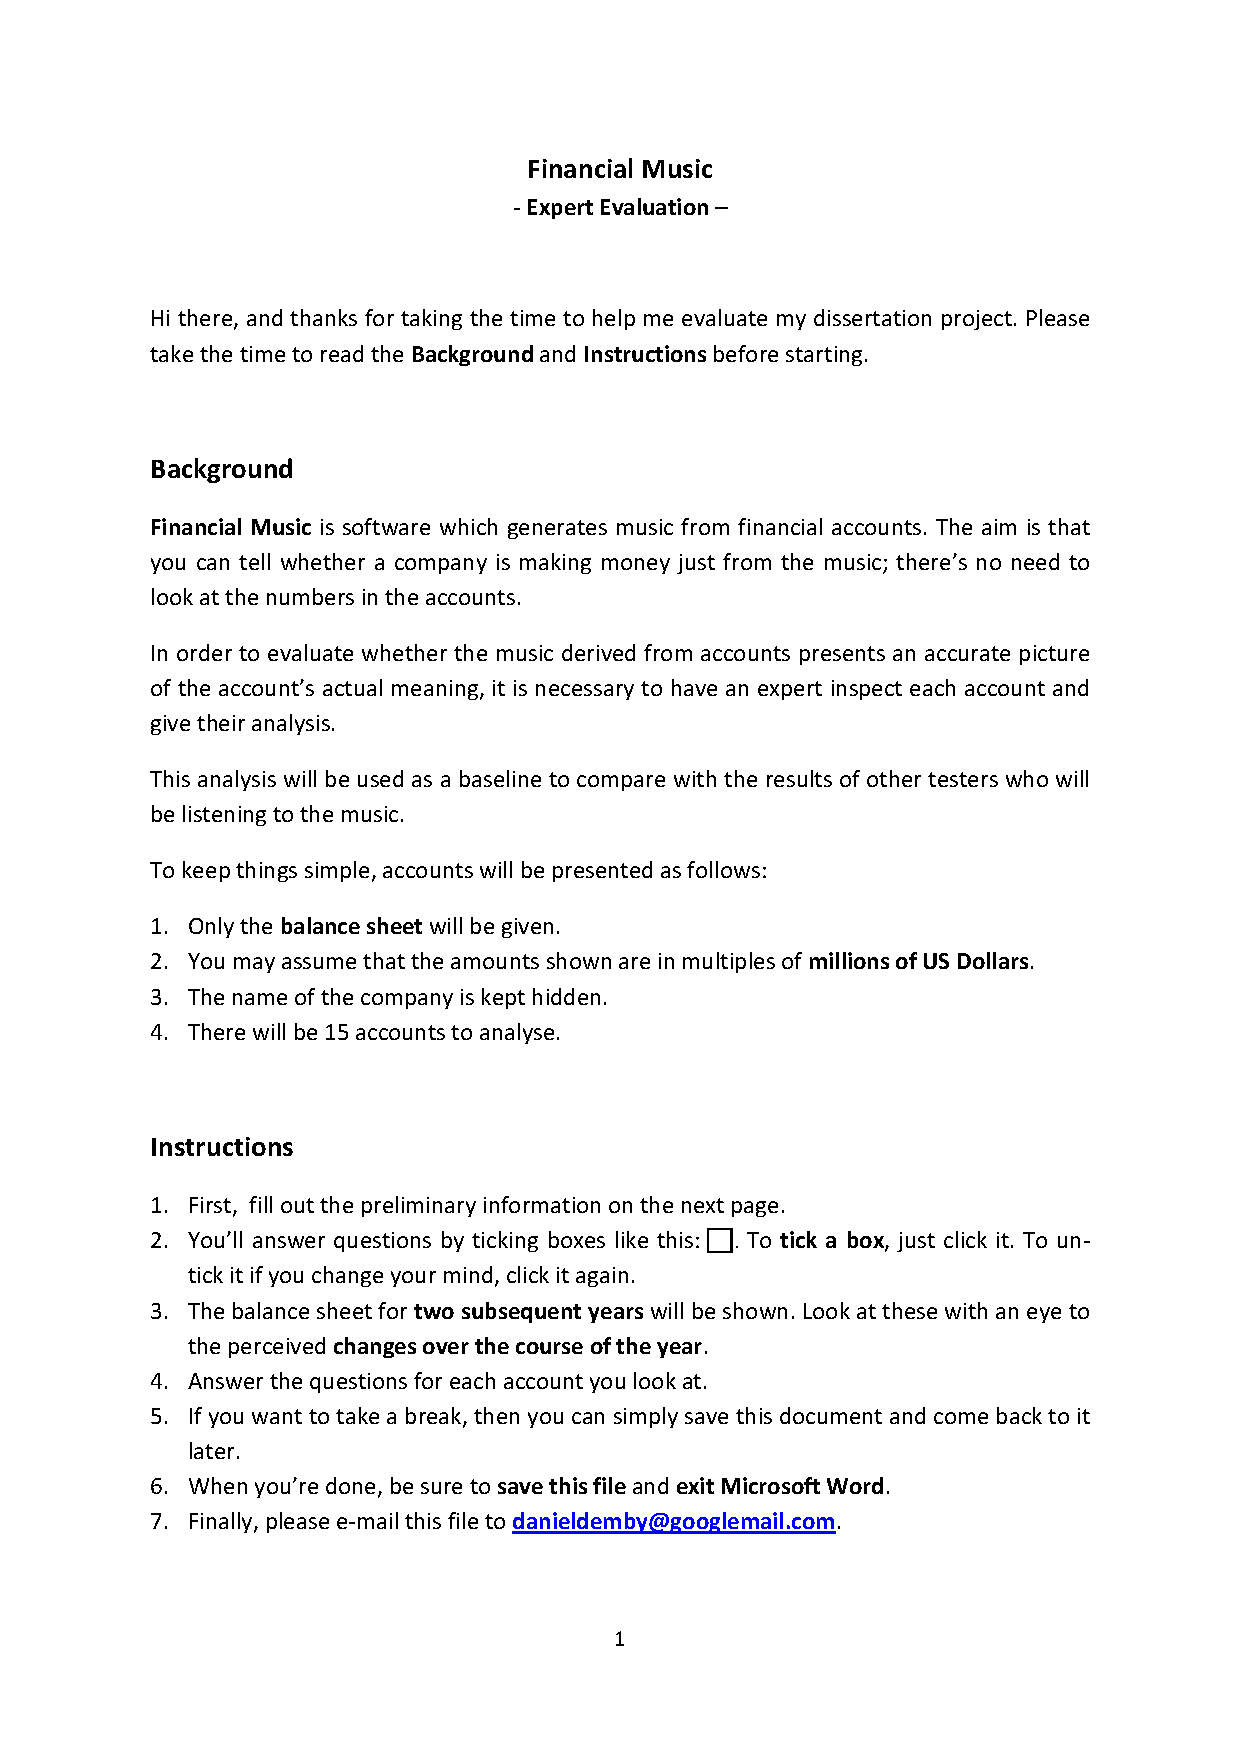
\includegraphics[scale=0.6]{qa1}
\caption{Page 1 of the expert's questionnaire.}
\label{fig:qa1}
\end{figure}

\begin{figure}[ht]
\centering
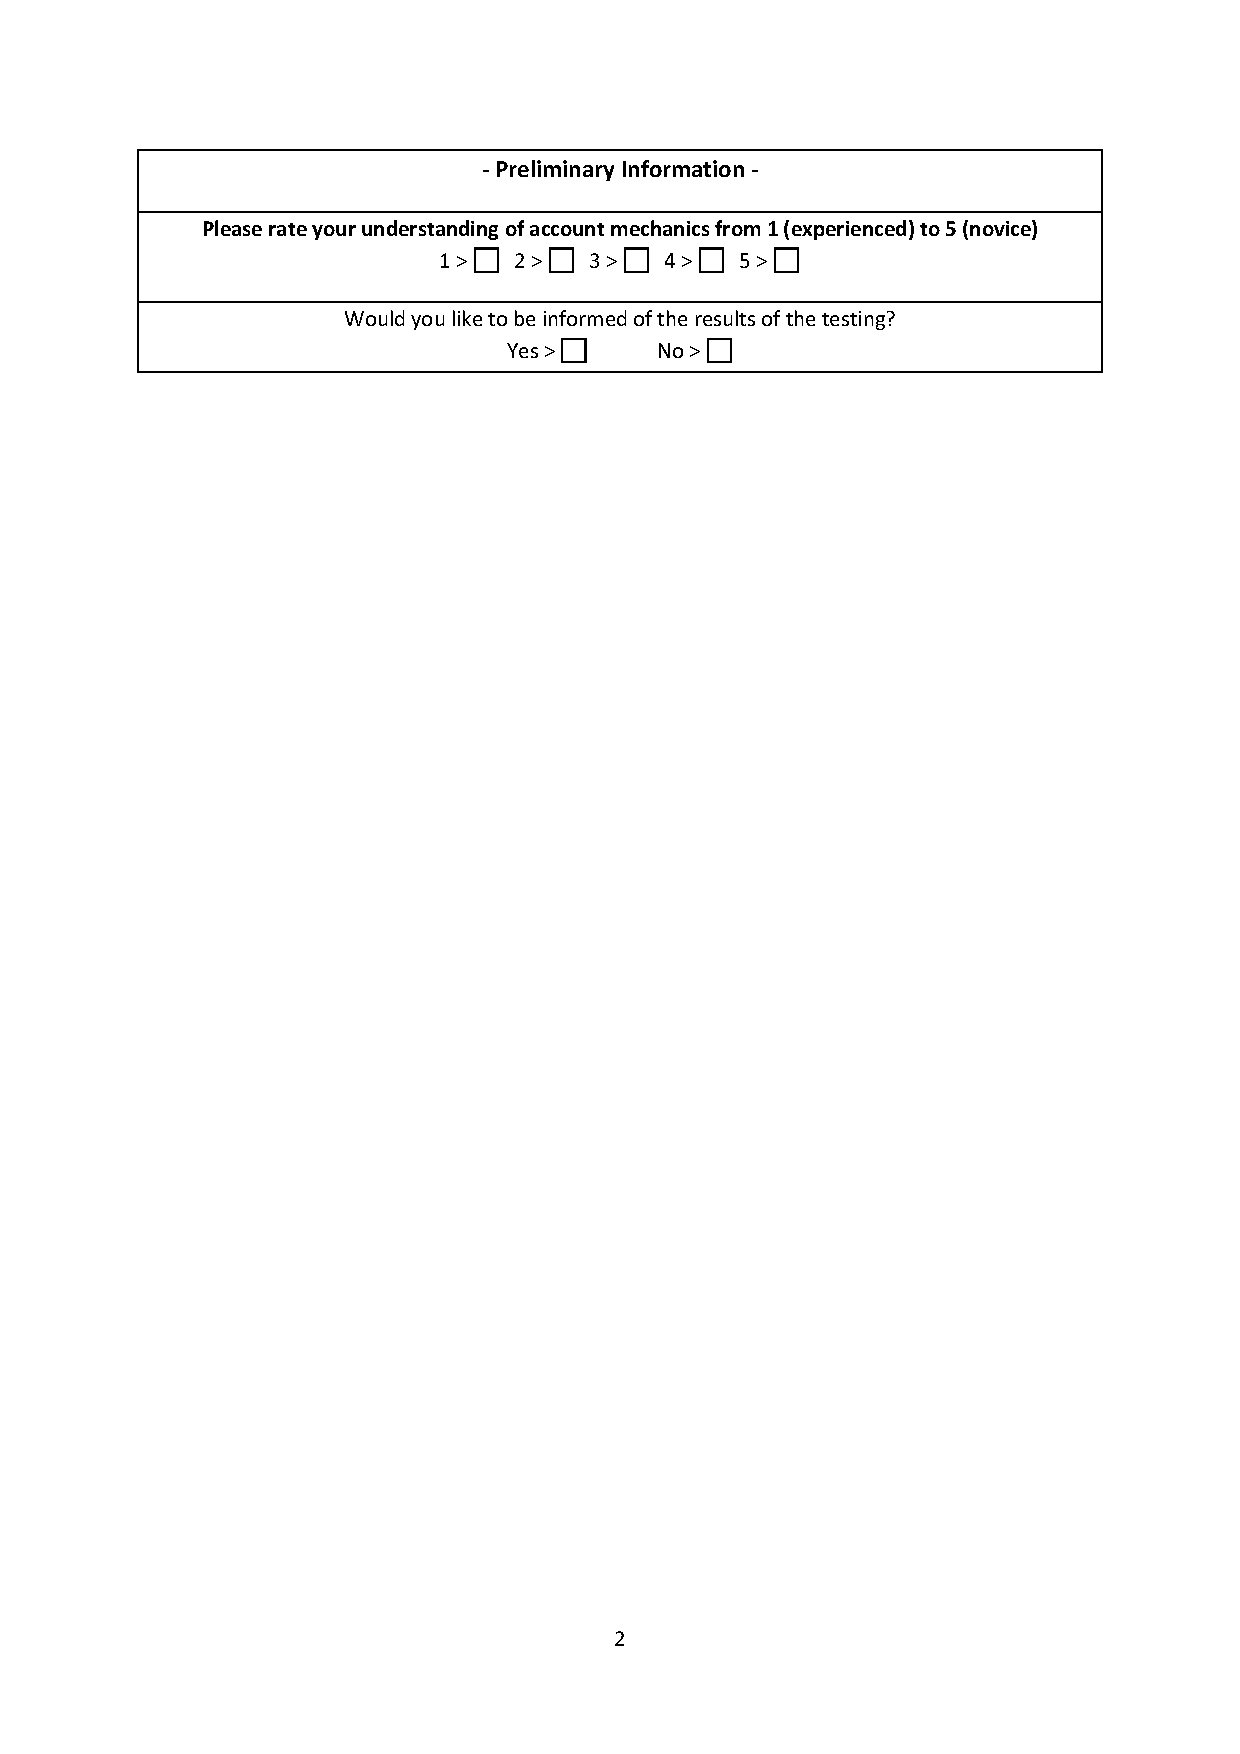
\includegraphics[scale=0.6]{qa2}
\caption{Page 2 of the expert's questionnaire.}
\label{fig:qa2}
\end{figure}

\begin{figure}[ht]
\centering
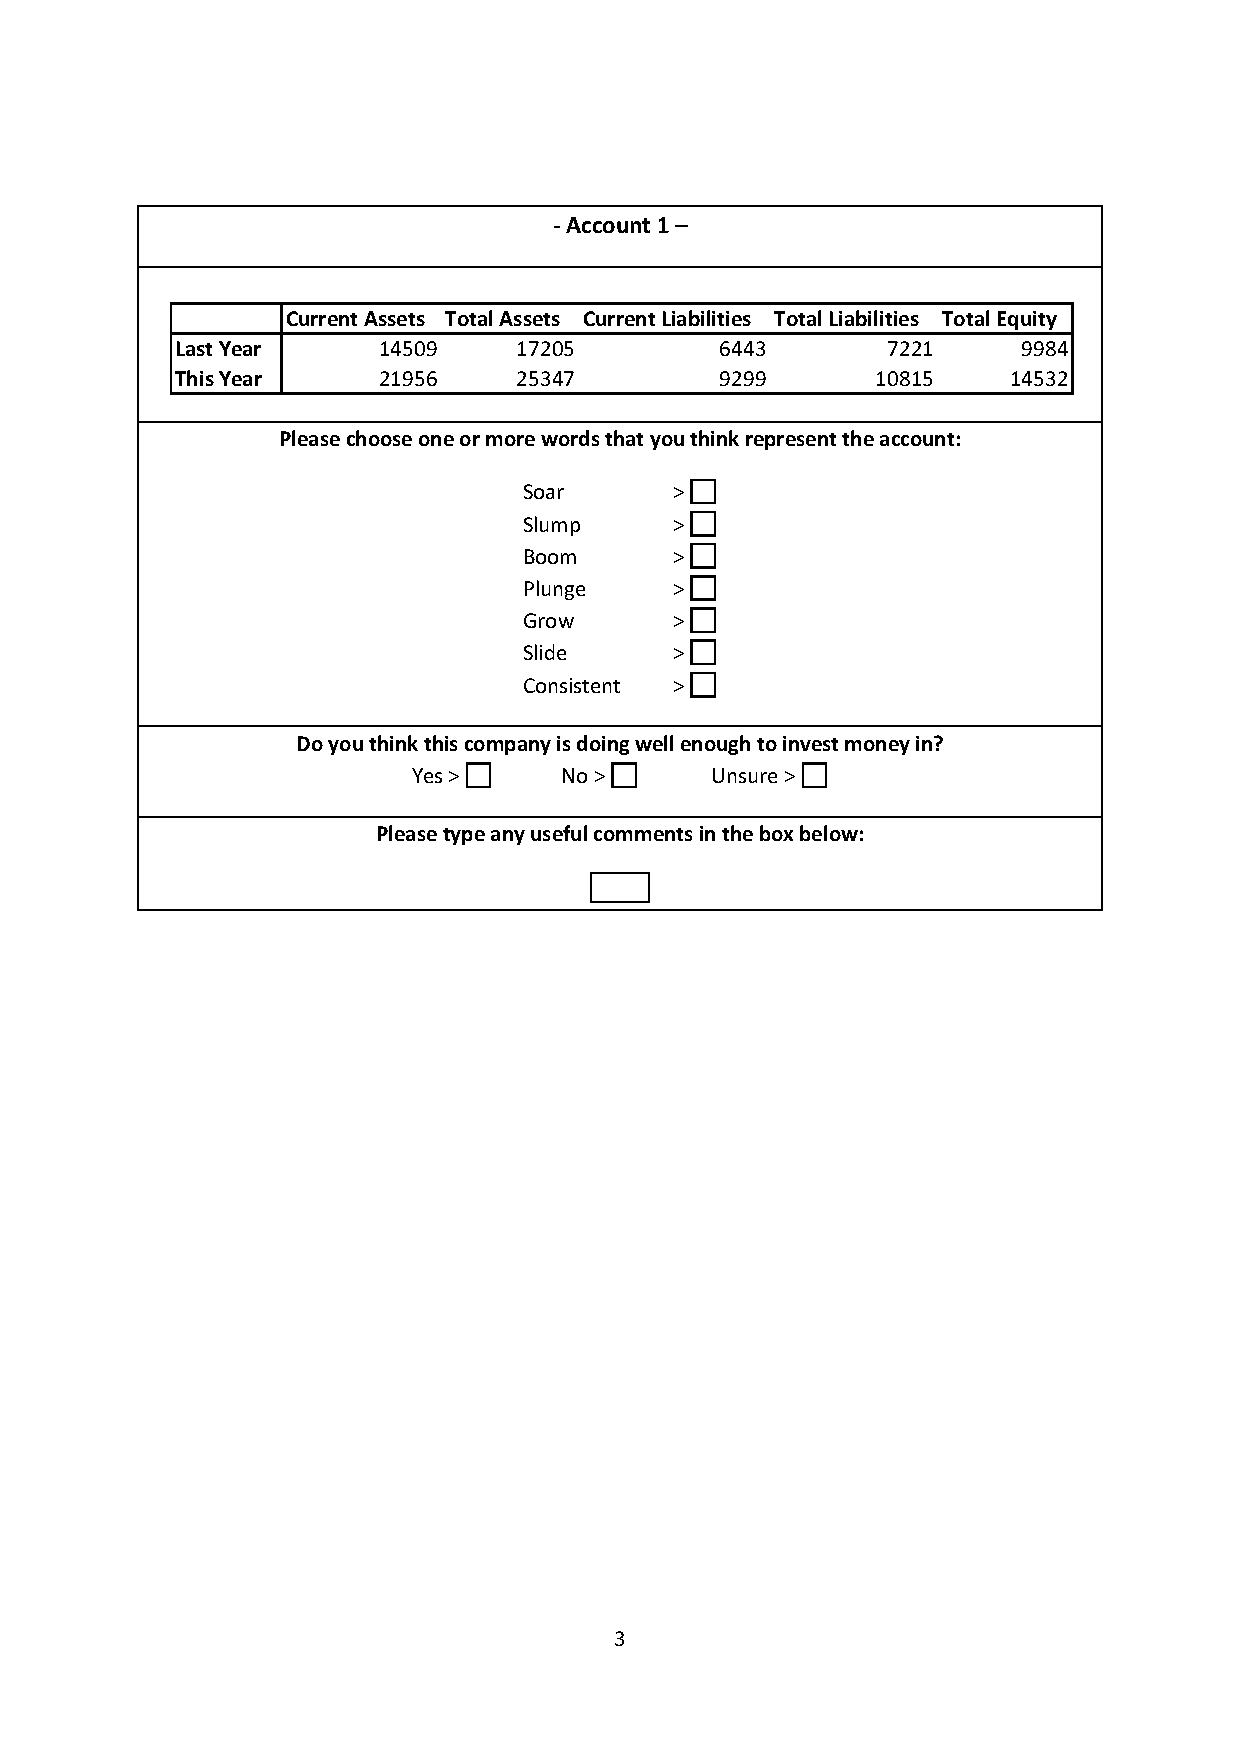
\includegraphics[scale=0.6]{qa3}
\caption{Page 3 of the expert's questionnaire. Future pages continue in the same fashion.}
\label{fig:qa3}
\end{figure}

\begin{figure}[ht]
\centering
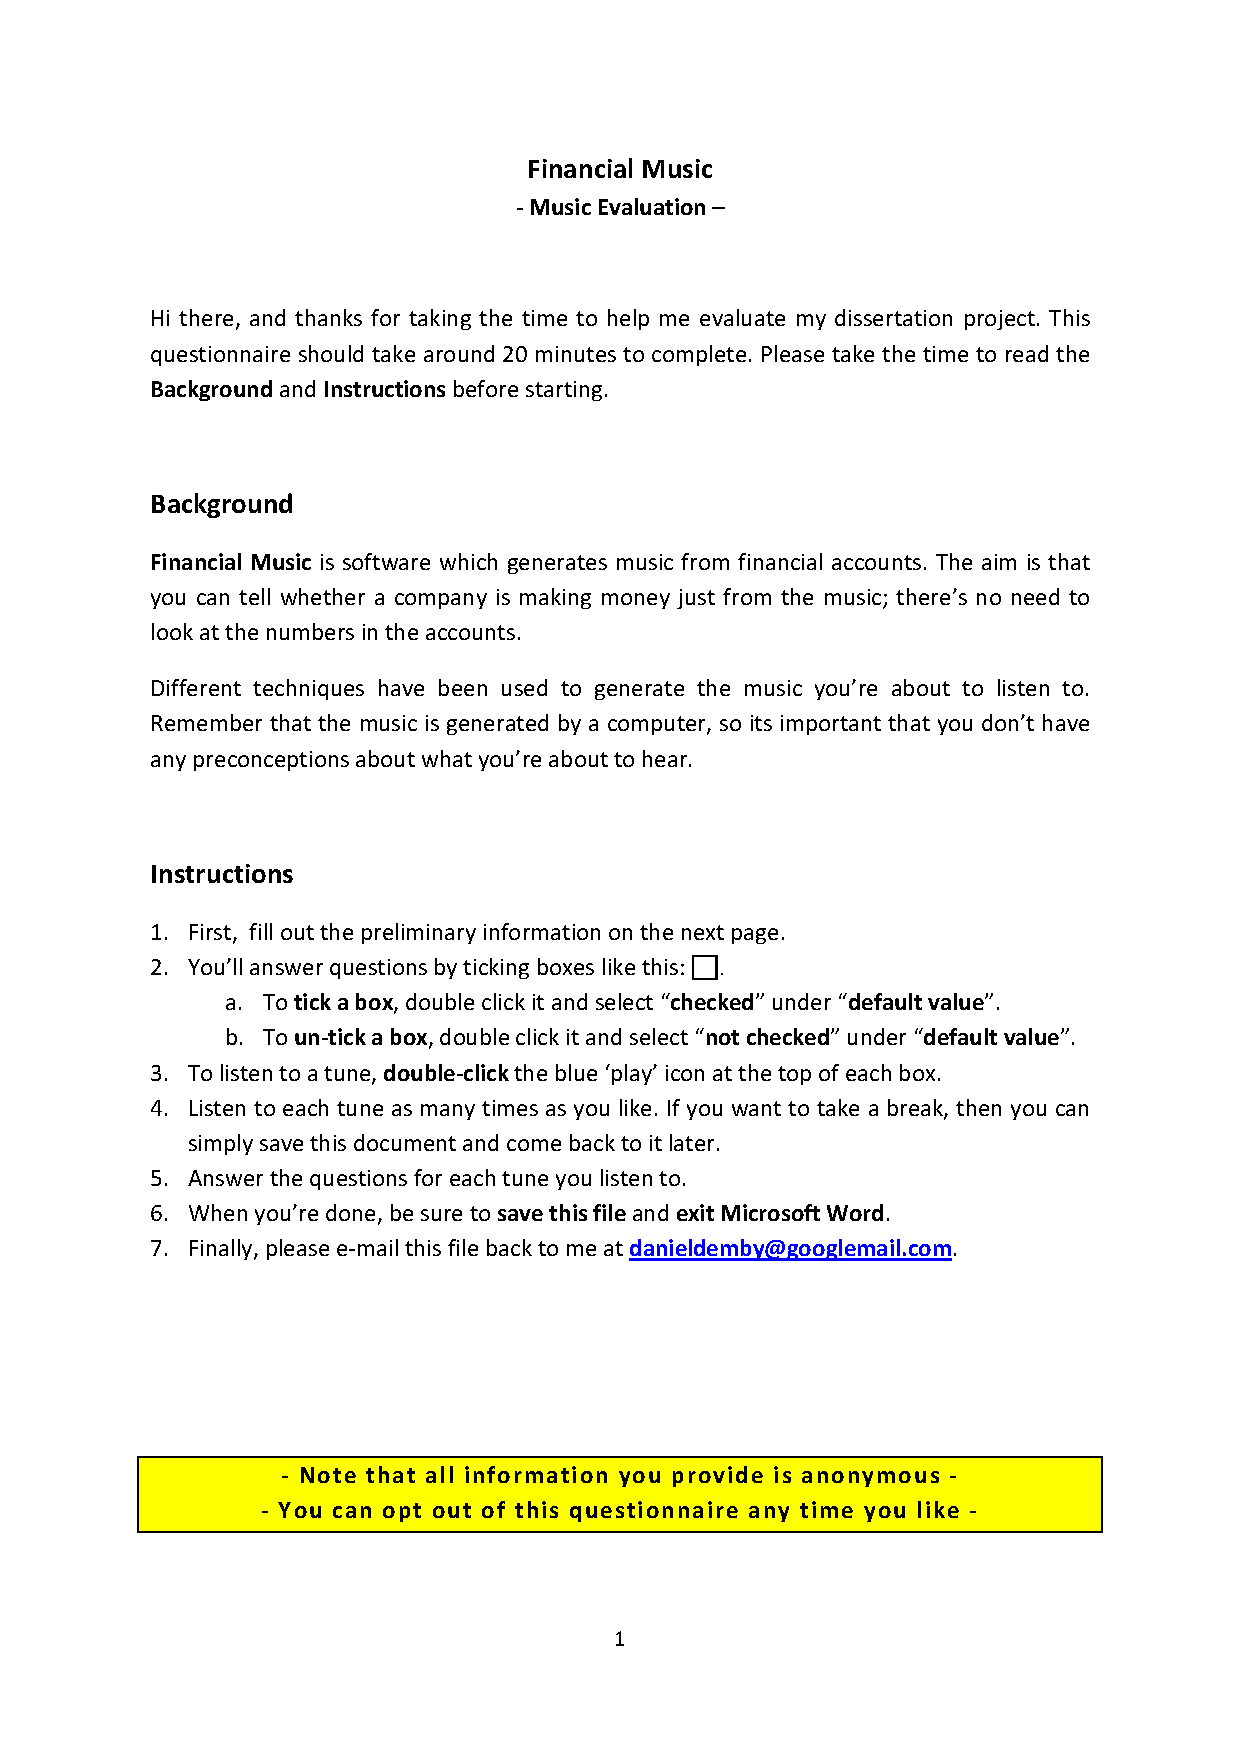
\includegraphics[scale=0.6]{qt1}
\caption{Page 1 of the tester's questionnaire.}
\label{fig:qt1}
\end{figure}

\begin{figure}[ht]
\centering
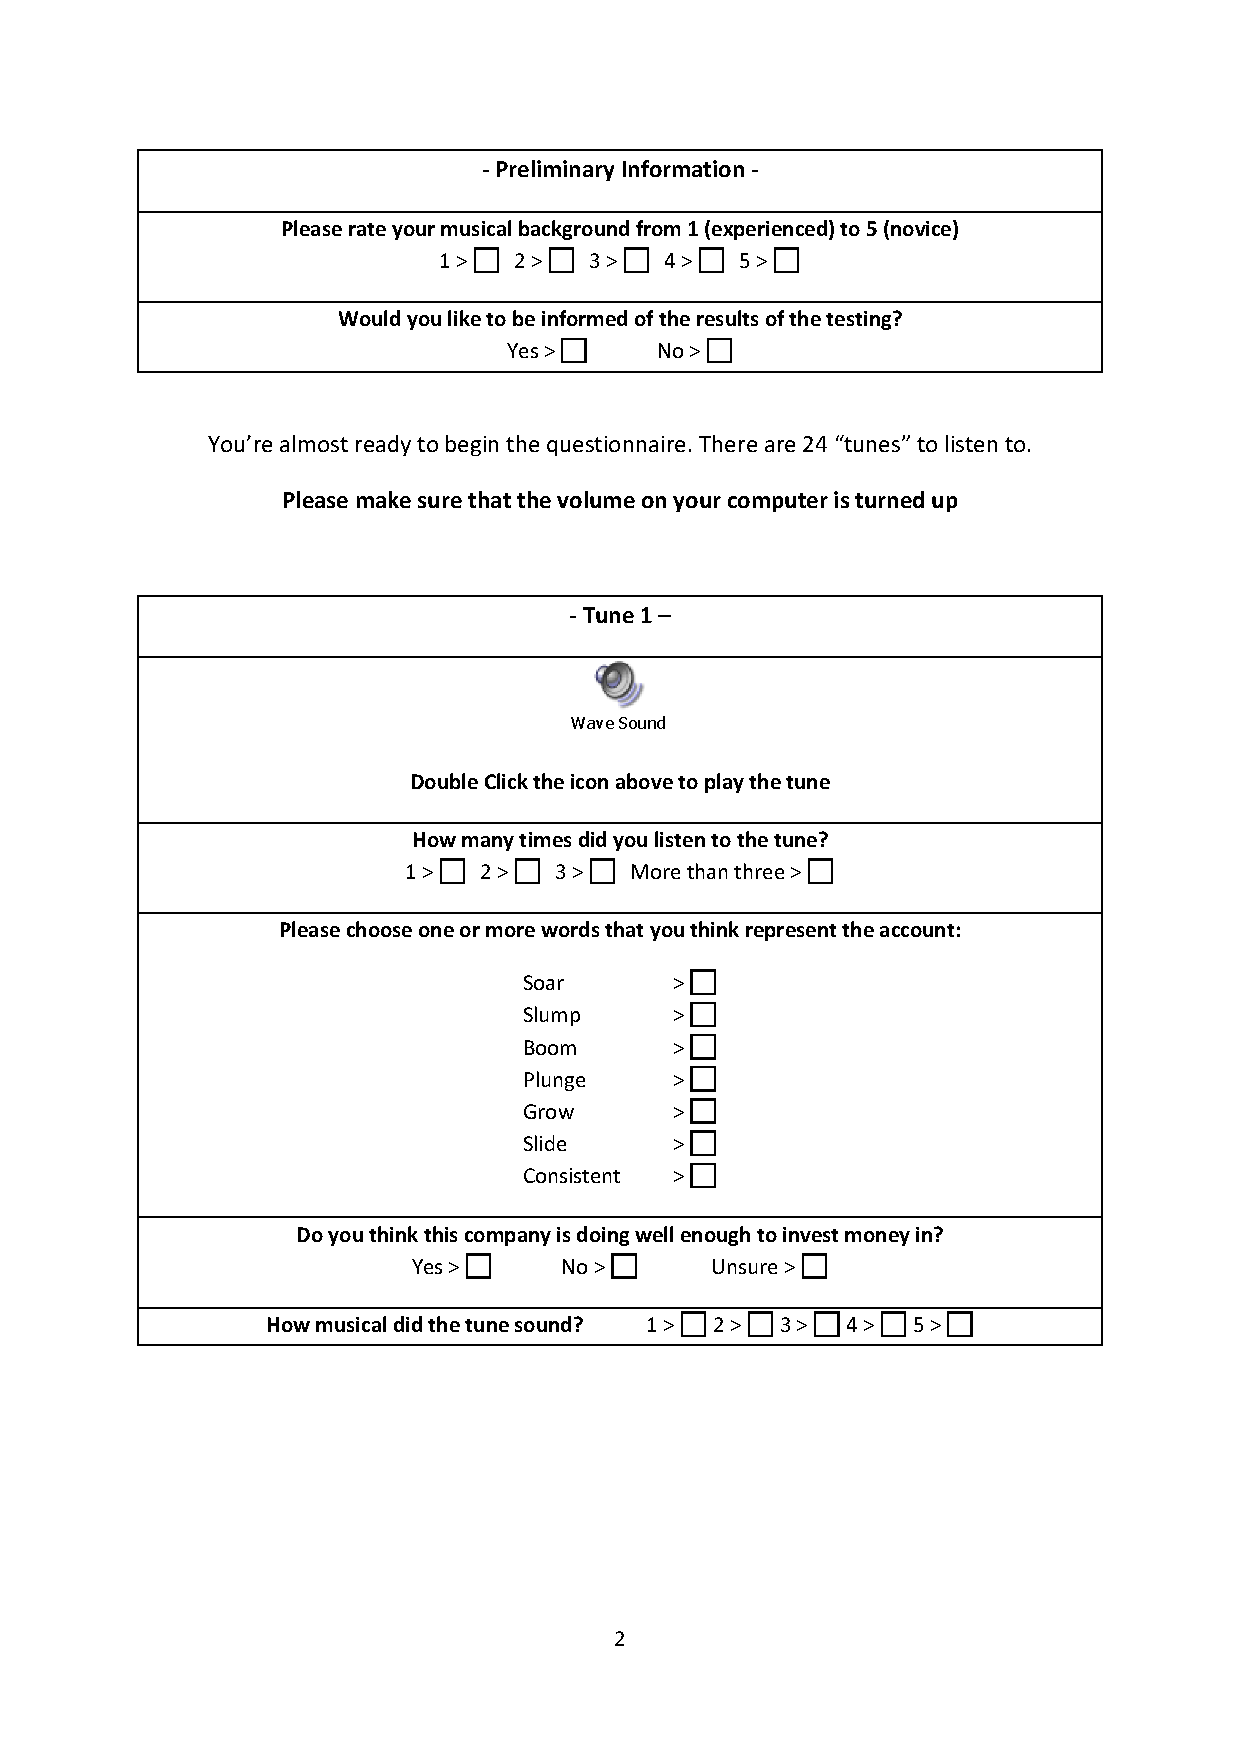
\includegraphics[scale=0.6]{qt2}
\caption{Page 2 of the tester's questionnaire. Future pages continue in the same fashion.}
\label{fig:qt2}
\end{figure}
\section{Appendix E: User Guide}

Welcome to the user guide. Here you will learn how to operate Financial Music.

\subsection*{System Requirements}

Before beginning, you will need to ensure you have Java 1.6 and Jython 2.2.1 installed. Java can be obtained from \url{www.sun.com} and Jython can be obtained from \url{www.jython.org}

\subsection*{File Formats}

Financial Music expects the account information to be in CSV (Comma Seperated Value) files. These can be opened or generated with a spreadsheet package such as Microsoft Excel.

\subsection*{Compiling Financial Music}

To prepare Financial Music for operation, you will need to open a command line console. Once this is done, navigate to the directory containing Financial music and type: \texttt{java *.java}. This will perform the compilation.

\subsection*{Music Generation}

Before generating the music, you will need to make sure that you have two subsequent years' balance sheets in two separate CSV files.\\

To generate music for the Signal Mapping implementation, type the following at the command line: \texttt{jython Mapping.py year1 year2}. Likewise, to generate music for the L-System Music Generation implementation, type: \texttt{jython LSS.py year1 year2}. In both instances, replace \texttt{year1} and \texttt{year2} with the appropriate file names.

\subsection*{Playing the Music}

Once the music is generated, you can hear it by typing the following at the command line: \texttt{java MusicReader}.

\subsection*{Changing Program Settings}

To alter the settings used to generate the music, open your favourite text editor and choose `open file'. Navigate to the Financial Music directory, and open \texttt{settings.py}. Within, you will find instructions on how to change these settings.
\section{Appendix F: Financial Genome Example}
\label{sec:genomeappend}
\subsection*{Full Genome}
\texttt{
16464   :  ['Boom', ['Descending', 'NULL', 'Chord']]\\
4200    :  ['Plunge', ['Descending', 'Minor', 'Scale']]\\
49392   :  ['Boom', ['Ascending', 'NULL', 'Chord']]\\
3430    :  ['Slump', ['NULL', 'Major', 'Chord']]\\
360     :  ['Plunge', ['Ascending', 'Major', 'NULL']]\\
82320   :  ['Boom', ['Descending', 'Major', 'Chord']]\\
8400    :  ['Boom', ['Descending', 'Minor', 'Scale']]\\
350     :  ['Slump', ['NULL', 'Minor', 'Scale']]\\
6860    :  ['Soar', ['NULL', 'Major', 'Chord']]\\
12600   :  ['Plunge', ['Ascending', 'Minor', 'Scale']]\\
720     :  ['Boom', ['Ascending', 'Major', 'NULL']]\\
336     :  ['Boom', ['Descending', 'NULL', 'Scale']]\\
10290   :  ['Slump', ['Descending', 'Major', 'Chord']]\\
1470    :  ['Slump', ['Descending', 'Major', 'Crescendo']]\\
700     :  ['Soar', ['NULL', 'Minor', 'Scale']]\\
13720   :  ['Plunge', ['NULL', 'Major', 'Chord']]\\
246960  :  ['Boom', ['Ascending', 'Major', 'Chord']]\\
25200   :  ['Boom', ['Ascending', 'Minor', 'Scale']]\\
4900    :  ['Soar', ['NULL', 'Minor', 'Crescendo']]\\
686     :  ['Slump', ['NULL', 'NULL', 'Chord']]\\
300     :  ['Soar', ['Descending', 'Minor', 'NULL']]\\
17150   :  ['Slump', ['NULL', 'Minor', 'Chord']]\\
294     :  ['Slump', ['Descending', 'NULL', 'Crescendo']]\\
29400   :  ['Plunge', ['Descending', 'Minor', 'Crescendo']]\\
4116    :  ['Soar', ['Descending', 'NULL', 'Chord']]\\
1050    :  ['Slump', ['Descending', 'Minor', 'Scale']]\\
20580   :  ['Soar', ['Descending', 'Major', 'Chord']]\\
280     :  ['Plunge', ['NULL', 'Major', 'Scale']]\\
11760   :  ['Boom', ['Descending', 'Major', 'Crescendo']]\\
1800    :  ['Plunge', ['Ascending', 'Minor', 'NULL']]\\
2940    :  ['Soar', ['Descending', 'Major', 'Crescendo']]\\
411600  :  ['Boom', ['Descending', 'Minor', 'Chord']]\\
102900  :  ['Soar', ['Descending', 'Minor', 'Chord']]\\
252     :  ['Soar', ['Ascending', 'NULL', 'Scale']]\\
1400    :  ['Plunge', ['NULL', 'Minor', 'Scale']]\\
630     :  ['Slump', ['Ascending', 'Major', 'Scale']]\\
27440   :  ['Boom', ['NULL', 'Major', 'Chord']]\\
1008    :  ['Boom', ['Ascending', 'NULL', 'Scale']]\\
240     :  ['Boom', ['Descending', 'Major', 'NULL']]\\
1764    :  ['Soar', ['Ascending', 'NULL', 'Crescendo']]\\
30870   :  ['Slump', ['Ascending', 'Major', 'Chord']]\\
9800    :  ['Plunge', ['NULL', 'Minor', 'Crescendo']]\\
1372    :  ['Soar', ['NULL', 'NULL', 'Chord']]\\
2520    :  ['Plunge', ['Ascending', 'Major', 'Scale']]\\
176400  :  ['Boom', ['Ascending', 'Minor', 'Crescendo']]\\
22050   :  ['Slump', ['Ascending', 'Minor', 'Crescendo']]\\
600     :  ['Plunge', ['Descending', 'Minor', 'NULL']]\\
980     :  ['Soar', ['NULL', 'Major', 'Crescendo']]\\
34300   :  ['Soar', ['NULL', 'Minor', 'Chord']]\\
210     :  ['Slump', ['Descending', 'Major', 'Scale']]\\
588     :  ['Soar', ['Descending', 'NULL', 'Crescendo']]\\
58800   :  ['Boom', ['Descending', 'Minor', 'Crescendo']]\\
200     :  ['Plunge', ['NULL', 'Minor', 'NULL']]\\
4410    :  ['Slump', ['Ascending', 'Major', 'Crescendo']]\\
196     :  ['Soar', ['NULL', 'NULL', 'Crescendo']]\\
8232    :  ['Plunge', ['Descending', 'NULL', 'Chord']]\\
2100    :  ['Soar', ['Descending', 'Minor', 'Scale']]\\
24696   :  ['Plunge', ['Ascending', 'NULL', 'Chord']]\\
180     :  ['Soar', ['Ascending', 'Major', 'NULL']]\\
41160   :  ['Plunge', ['Descending', 'Major', 'Chord']]\\
560     :  ['Boom', ['NULL', 'Major', 'Scale']]\\
6300    :  ['Soar', ['Ascending', 'Minor', 'Scale']]\\
168     :  ['Plunge', ['Descending', 'NULL', 'Scale']]\\
7056    :  ['Boom', ['Ascending', 'NULL', 'Crescendo']]\\
123480  :  ['Plunge', ['Ascending', 'Major', 'Chord']]\\
3600    :  ['Boom', ['Ascending', 'Minor', 'NULL']]\\
2450    :  ['Slump', ['NULL', 'Minor', 'Crescendo']]\\
150     :  ['Slump', ['Descending', 'Minor', 'NULL']]\\
1680    :  ['Boom', ['Descending', 'Major', 'Scale']]\\
14700   :  ['Soar', ['Descending', 'Minor', 'Crescendo']]\\
144     :  ['Boom', ['Ascending', 'NULL', 'NULL']]\\
2058    :  ['Slump', ['Descending', 'NULL', 'Chord']]\\
140     :  ['Soar', ['NULL', 'Major', 'Scale']]\\
5880    :  ['Plunge', ['Descending', 'Major', 'Crescendo']]\\
900     :  ['Soar', ['Ascending', 'Minor', 'NULL']]\\
205800  :  ['Plunge', ['Descending', 'Minor', 'Chord']]\\
51450   :  ['Slump', ['Descending', 'Minor', 'Chord']]\\
126     :  ['Slump', ['Ascending', 'NULL', 'Scale']]\\
5488    :  ['Boom', ['NULL', 'NULL', 'Chord']]\\
504     :  ['Plunge', ['Ascending', 'NULL', 'Scale']]\\
120     :  ['Plunge', ['Descending', 'Major', 'NULL']]\\
2800    :  ['Boom', ['NULL', 'Minor', 'Scale']]\\
882     :  ['Slump', ['Ascending', 'NULL', 'Crescendo']]\\
112     :  ['Boom', ['NULL', 'NULL', 'Scale']]\\
1260    :  ['Soar', ['Ascending', 'Major', 'Scale']]\\
88200   :  ['Plunge', ['Ascending', 'Minor', 'Crescendo']]\\
490     :  ['Slump', ['NULL', 'Major', 'Crescendo']]\\
100     :  ['Soar', ['NULL', 'Minor', 'NULL']]\\
98      :  ['Slump', ['NULL', 'NULL', 'Crescendo']]\\
12348   :  ['Soar', ['Ascending', 'NULL', 'Chord']]\\
90      :  ['Slump', ['Ascending', 'Major', 'NULL']]\\
3920    :  ['Boom', ['NULL', 'Major', 'Crescendo']]\\
137200  :  ['Boom', ['NULL', 'Minor', 'Chord']]\\
3150    :  ['Slump', ['Ascending', 'Minor', 'Scale']]\\
84      :  ['Soar', ['Descending', 'NULL', 'Scale']]\\
3528    :  ['Plunge', ['Ascending', 'NULL', 'Crescendo']]\\
80      :  ['Boom', ['NULL', 'Major', 'NULL']]\\
61740   :  ['Soar', ['Ascending', 'Major', 'Chord']]\\
840     :  ['Plunge', ['Descending', 'Major', 'Scale']]\\
7350    :  ['Slump', ['Descending', 'Minor', 'Crescendo']]\\
72      :  ['Plunge', ['Ascending', 'NULL', 'NULL']]\\
70      :  ['Slump', ['NULL', 'Major', 'Scale']]\\
450     :  ['Slump', ['Ascending', 'Minor', 'NULL']]\\
19600   :  ['Boom', ['NULL', 'Minor', 'Crescendo']]\\
2744    :  ['Plunge', ['NULL', 'NULL', 'Chord']]\\
5040    :  ['Boom', ['Ascending', 'Major', 'Scale']]\\
60      :  ['Soar', ['Descending', 'Major', 'NULL']]\\
56      :  ['Plunge', ['NULL', 'NULL', 'Scale']]\\
44100   :  ['Soar', ['Ascending', 'Minor', 'Crescendo']]\\
2352    :  ['Boom', ['Descending', 'NULL', 'Crescendo']]\\
1200    :  ['Boom', ['Descending', 'Minor', 'NULL']]\\
50      :  ['Slump', ['NULL', 'Minor', 'NULL']]\\
48      :  ['Boom', ['Descending', 'NULL', 'NULL']]\\
6174    :  ['Slump', ['Ascending', 'NULL', 'Chord']]\\
1960    :  ['Plunge', ['NULL', 'Major', 'Crescendo']]\\
35280   :  ['Boom', ['Ascending', 'Major', 'Crescendo']]\\
68600   :  ['Plunge', ['NULL', 'Minor', 'Chord']]\\
42      :  ['Slump', ['Descending', 'NULL', 'Scale']]\\
40      :  ['Plunge', ['NULL', 'Major', 'NULL']]\\
420     :  ['Soar', ['Descending', 'Major', 'Scale']]\\
36      :  ['Soar', ['Ascending', 'NULL', 'NULL']]\\
30      :  ['Slump', ['Descending', 'Major', 'NULL']]\\
28      :  ['Soar', ['NULL', 'NULL', 'Scale']]\\
1176    :  ['Plunge', ['Descending', 'NULL', 'Crescendo']]\\
24      :  ['Plunge', ['Descending', 'NULL', 'NULL']]\\
17640   :  ['Plunge', ['Ascending', 'Major', 'Crescendo']]\\
20      :  ['Soar', ['NULL', 'Major', 'NULL']]\\
18      :  ['Slump', ['Ascending', 'NULL', 'NULL']]\\
784     :  ['Boom', ['NULL', 'NULL', 'Crescendo']]\\
400     :  ['Boom', ['NULL', 'Minor', 'NULL']]\\
16      :  ['Boom', ['NULL', 'NULL', 'NULL']]\\
14      :  ['Slump', ['NULL', 'NULL', 'Scale']]\\
12      :  ['Soar', ['Descending', 'NULL', 'NULL']]\\
8820    :  ['Soar', ['Ascending', 'Major', 'Crescendo']]\\
10      :  ['Slump', ['NULL', 'Major', 'NULL']]\\
392     :  ['Plunge', ['NULL', 'NULL', 'Crescendo']]\\
1234800 :  ['Boom', ['Ascending', 'Minor', 'Chord']]\\
8       :  ['Plunge', ['NULL', 'NULL', 'NULL']]\\
6       :  ['Slump', ['Descending', 'NULL', 'NULL']]\\
4       :  ['Soar', ['NULL', 'NULL', 'NULL']]\\
617400  :  ['Plunge', ['Ascending', 'Minor', 'Chord']]\\
2       :  ['Slump', ['NULL', 'NULL', 'NULL']]\\
308700  :  ['Soar', ['Ascending', 'Minor', 'Chord']]\\
154350  :  ['Slump', ['Ascending', 'Minor', 'Chord']]}\\

\subsection*{Vailid Genes}

\texttt{
58800   :  ['Boom', ['Descending', 'Minor', 'Crescendo']]\\
2940    :  ['Soar', ['Descending', 'Major', 'Crescendo']]\\
5880    :  ['Plunge', ['Descending', 'Major', 'Crescendo']]\\
8820    :  ['Soar', ['Ascending', 'Major', 'Crescendo']]\\
176400  :  ['Boom', ['Ascending', 'Minor', 'Crescendo']]\\
27440   :  ['Boom', ['NULL', 'Major', 'Chord']]\\
840     :  ['Plunge', ['Descending', 'Major', 'Scale']]\\
11760   :  ['Boom', ['Descending', 'Major', 'Crescendo']]\\
14700   :  ['Soar', ['Descending', 'Minor', 'Crescendo']]\\
17640   :  ['Plunge', ['Ascending', 'Major', 'Crescendo']]\\
1680    :  ['Boom', ['Descending', 'Major', 'Scale']]\\
12600   :  ['Plunge', ['Ascending', 'Minor', 'Scale']]\\
630     :  ['Slump', ['Ascending', 'Major', 'Scale']]\\
2520    :  ['Plunge', ['Ascending', 'Major', 'Scale']]\\
17150   :  ['Slump', ['NULL', 'Minor', 'Chord']]\\
1470    :  ['Slump', ['Descending', 'Major', 'Crescendo']]\\
29400   :  ['Plunge', ['Descending', 'Minor', 'Crescendo']]\\
420     :  ['Soar', ['Descending', 'Major', 'Scale']]\\
88200   :  ['Plunge', ['Ascending', 'Minor', 'Crescendo']]\\
8400    :  ['Boom', ['Descending', 'Minor', 'Scale']]\\
4410    :  ['Slump', ['Ascending', 'Major', 'Crescendo']]\\
13720   :  ['Plunge', ['NULL', 'Major', 'Chord']]\\
35280   :  ['Boom', ['Ascending', 'Major', 'Crescendo']]\\
7350    :  ['Slump', ['Descending', 'Minor', 'Crescendo']]\\
6300    :  ['Soar', ['Ascending', 'Minor', 'Scale']]\\
25200   :  ['Boom', ['Ascending', 'Minor', 'Scale']]\\
1260    :  ['Soar', ['Ascending', 'Major', 'Scale']]\\
137200  :  ['Boom', ['NULL', 'Minor', 'Chord']]\\
44100   :  ['Soar', ['Ascending', 'Minor', 'Crescendo']]\\
4200    :  ['Plunge', ['Descending', 'Minor', 'Scale']]\\
210     :  ['Slump', ['Descending', 'Major', 'Scale']]\\
6860    :  ['Soar', ['NULL', 'Major', 'Chord']]\\
3150    :  ['Slump', ['Ascending', 'Minor', 'Scale']]\\
68600   :  ['Plunge', ['NULL', 'Minor', 'Chord']]\\
22050   :  ['Slump', ['Ascending', 'Minor', 'Crescendo']]\\
2100    :  ['Soar', ['Descending', 'Minor', 'Scale']]\\
3430    :  ['Slump', ['NULL', 'Major', 'Chord']]\\
5040    :  ['Boom', ['Ascending', 'Major', 'Scale']]\\
1050    :  ['Slump', ['Descending', 'Minor', 'Scale']]\\
34300   :  ['Soar', ['NULL', 'Minor', 'Chord']]\\
40  out of  144  genes are valid.}
\section{Appendix G: Progress Log}

This log details the progress of my dissertation through its final few weeks. The purpose of the log is to provide evidence of the work that has applied to the task, just in case the worse should happen (such as all the departmental servers melting at the same time as my laptop explodes, setting fire to all printed documents in the vicinity).

I think its fair to say that as Deliverables 1 \& 2 are now a matter of record. These in themselves provide adequate evidence of work achieved over the earlier sections of the project.

(Each day's entries were written as I was working, so the tenses may fluctuate between past, present and future!)
\end{singlespace}

% Generic figure template
%\begin{figure}[ht]
%\centering
%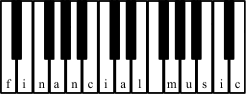
\includegraphics[scale=0.75]{logo}
%\caption{A graph showing the average amount that testers agreed with the expert's decision whether to invest in an account, not invest in an account or to remain undecided.}
%\label{fig:agreegraph}
%\end{figure}

\end{document}